\documentclass[12pt,brazil]{book}
\usepackage{babel}
\usepackage[utf8x]{inputenc}
\usepackage[top=2.5cm,left=2.5cm,bottom=2.5cm,right=2.5cm]{geometry}
\usepackage{url}
\usepackage{graphicx}
\usepackage{html}


\newcommand{\sep}{$\rightarrow$}
\newcommand{\eng}[1]{\textit{#1}}
\newcommand{\code}[1]{\texttt{#1}}

\title{Genoslab Handbook}
\author{Pedro Kröger, Marcos di Silva e Alexandre Passos}

\begin{document}
\graphicspath{{figs/}}

\maketitle

\begin{htmlonly}
  Baixe a versão em pdf \htmladdnormallink{aqui}
  {http://genos.mus.br/handbook/genoslab-handbook.pdf}.
\end{htmlonly}

\tableofcontents

\part{Introdução}
\label{part:introducao}

\chapter{Programas no genoslab}
\label{cha:progr-no-genosl}

Basic infrastructure
      alsa-tools - Console based ALSA utilities for specific hardware
      alsa-tools-gui - GUI based ALSA utilities for specific hardware
      linux-image-rt - Low latency kernel
      qamix - Configurable mixer for ALSA

JACK and JACK Utilities
      jackd - JACK Audio Connection Kit (server and example clients)
      qjackctl - User interface for controlling the JACK sound server
      bitscope - diagnosis tool for JACK audio software
      jdelay - A small command line JACK app you can use to measure the latency of your sound card.
      meterbridge - A collection of Audio meters for the JACK audio server
      patchage - modular patch bay for Jack audio and Alsa Midi
      jack-tools - various JACK tools: plumbing, play, udp, ctl, scope, clock

Sound editing and recording
      audacity - Swiss army audio editor
      timemachine - JACK audio recorder for spontaneous and conservatory use

Audio playback
      xmms - Versatile X audio player
      xmms-jackasyn - JACK Output plugin for xmms
      xmms-modplug - ModPlug plugin for XMMS

Digital Audio Workstation software
      ardour - Digital audio workstation (graphical gtk interface)
      beast - music synthesis and composition framework

Synthesizers
      fluidsynth - Real-time MIDI software synthesizer
      bristol - vintage synthesizer emulator
      freebirth - Bass synthesizer/sample player/sequencer similar to Rebirth
      qsynth - fluidsynth MIDI sound synthesiser front-end
      zynaddsubfx - Realtime software synthesizer for Linux
      csound - powerful and versatile sound synthesis software
      swami - SoundFont editor

Sampling
      linuxsampler - software audio sampler
      sooperlooper - Looping Sampler LADSPA plugin

Sequencing
      aconnectgui - graphical ALSA sequencer connection manager
      rosegarden4 - music editor and MIDI/audio sequencer
      hydrogen - Simple drum machine/step sequencer
      seq24 - Real time MIDI sequencer
      jackbeat - audio sequencer
      muse - Qt-based midi/audio sequencer
      tk707 - drum sequencer for a sound card or MIDI device
      shaketracker - MIDI sequencer with tracker GUI

Effects and signal processing
      jack-rack - LADSPA effects "rack" for JACK
      tapiir - A tool for real time audio delay and feedback effects
      freqtweak - Realtime audio frequency spectral manipulation
      jamin - Audio mastering from a mixed down multitrack source with JACK
      creox - real-time guitar effects
      jackeq - routes and manipulates audio from/to multiple sources

DJ tools
      terminatorx - A realtime audio synthesizer
      mixxx - A digital DJ interface (for beat-mixing)

MIDI Utilities
      timidity - Software sound renderer (MIDI sequencer, MOD player)
      vkeybd - Virtual Keyboard program

Musical typesetting
      denemo - A gtk+ frontend to GNU Lilypond
      lilypond-data - LilyPond music typesetter (data files)
      lilypond - A program for typesetting sheet music

Miscellaneous / uncategorized
      gtick - Metronome application
      puredata - realtime computer music and graphics system
      audatious -

ubuntustudio-plugins

A plug-ins package.
Package list:

aeolus blop caps cmt hexter fil-plugins ladspa-sdk mcp-plugins omins swh-plugins tap-plugins vcf dssi-example-plugins dssi-host-jack fluidsynth-dssi xsynth-dssi dssi-utils
Description:

      aeolus - Aeolus is a synthesized (i.e. not sampled) pipe organ emulator
      blop - Bandlimited wavetable-based oscillator plugins for LADSPA hosts.
      caps - A collection of refined LADSPA plugins.
      cmt - (Computer Music Toolkit) A collection of LADSPA compatible plugins.
      fil-plugins - Parametric equalizer LADSPA plugin.
      hexter - Yamaha DX7 modeling DSSI plugin
      ladspa-sdk - Sample tools for linux-audio-dev plugin architecture.
      mcp-plugins - LADSPA plugins designed for Alsa Modular Synth.
      omins - Collection of LADSPA plugins geared at modular synthesizers.
      swh-plugins - Steve Harris's LADSPA plugins.
      tap-plugins - Tom's Audio Processing LADSPA plugins.
      vcf - Audio EQ biquad filter LADSPA plugins.
      dssi-example-plugins - Example DSSI plugins.
      dssi-host-jack - An example DSSI host.
      fluidsynth-dssi - Soundfont player/synth for DSSI.
      xsynth-dssi - A classic-analog style softsynth DSSI plugin.
      dssi-utils - Command-line utilities for sending commands to DSSI plugins.

ubuntustudio-video

Video editing apps.
Package list:

openmovieeditor ffmpeg ffmpeg2theora kino stopmotion synfigstudio dvgrab
Description:

      openmovieeditor - Video editor
      ffmpeg - Multimedia player, server and encoder
      ffmpeg2theora - Theora video encoder using ffmpeg
      kino - A non-linear editor for Digital Video data
      stopmotion - A program for creating stop motion animation.
      dvgrab - Grab digital video data via IEEE1394 links

ubuntustudio-graphics

A current, complete set of 2D/3D manipulation applications. ie: Inkscape, GIMP, Blender, and so on.
Package list:

inkscape blender gimp gimp-gap gimp-ufraw gimp-plugin-registry f-spot scribus fontforge gnome-raw-thumbnailer xsane wacom-tools hugin agave yafray
Description:

      inkscape - A vector-based drawing program.
      blender - A very fast and versatile 3D suite for modeling, animation, rendering, post-production, interactive creation and playback.
      gimp - A raster-based drawing program.
      gimp-gap - GAP is a collection of plug-ins to extend the GIMP with capabilities to edit and create animations and movies as sequences of single frames.
      gimp-print - Print plugin for the GIMP
      gimp-ufraw - A plug-in to import RAW images.
      gimp-plugin-registry - A collection of GIMP plugins.
      f-spot - A personal photo management application.
      scribus - A open source desktop page layout program.
      fontforge - Font Editor for PS, TrueType and OpenType fonts.
      gnome-raw-thumbnailer - a thumbnailer for GNOME that will make thumbnails for camera RAW files.
      xsane - GTK+-based X11 frontend for SANE. (Scanner Access Now Easy)
      wacom-tools - Software for you Wacom drawing pad.
      hugin - An easy to use cross-platform GUI for Panorama Tools.
      synfigstudio - A vector 2D based animation package (GUI)
      agave - Colorscheme generator.
      enblend - A tool for compositing images.
      yafray - A modern, xml-speaking raytracing-based rendering system
      nautilus-image-converter - nautilus extension to mass resize images


\chapter{Como contribuir para esse documento}
\label{sec:como-contribuir-para}

\part{Guia para membros do Genos}
\label{part:guia-para-membros}

\chapter{As ferramentas on-line do genos}
\label{cha:ferramentas-genos}

\section{Editando o wiki off-line com git}
\label{sec:editando-o-wiki}

Você pode baixar o wiki para o seu computador com o git, fazer
modificações e enviar de volta para o servidor. Por exemplo, para
editar a página principal do wiki:

\begin{verbatim}
git clone git@genos.mus.br:genos-wiki
cd genos-wiki
... edita index.mdwn ...
git add index.mdwn
git commit -m "acrescenta mais texto"
git push
\end{verbatim}

Contudo, se você vai trabalhar bastante no wiki é mais prático ter uma
cópia local do wiki para você acompanhar as mudanças sem ter que
envia-las para o repositório central. Isso é particularmente útil para
modificar o estilo css.

Primeiramente você precisa instalar o ikiwiki e um servidor web no seu
computador. O lighttpd é uma alternativa leve e rápida ao Apache.

\begin{verbatim}
pacman -S ikiwiki lighttpd
\end{verbatim}

Além disso é necessário instalar alguns pacotes de perl para que
alguns plugins do ikiwiki funcionem:

\begin{verbatim}
pacman -S perl-net-openid-consumer xapian-omega perl-crypt-dh \
          perl-search-xapian perl-paranoid perl-crypt-ssleay \
          perl-libwww perl-uri-fetch perl-digest-sha1 \
          perl-html-scrubber xapian-core 
\end{verbatim}

O próximo passo é configurar o lighttpd. Acrescente as seguintes
linhas no arquivo de configuração em
\url{/etc/lighttpd/lighttpd.conf}:

\begin{verbatim}
userdir.path = "public_html"
cgi.assign = ( "ikiwiki.cgi" => "")
\end{verbatim}

Além disso garanta que os seguintes modulos estão ativados no arquivo
de configuração do lighttpd (eles estão ativados se não tiverem um
``\#'' na linha):

\begin{verbatim}
server.modules = ("mod_access",
                  "mod_userdir",
                  "mod_cgi",
                  "mod_usertrack",
                  "mod_accesslog" )
\end{verbatim}

Reinicie o lighttpd com \code{/etc/rc.d/lighttpd restart} ou
\code{/etc/init.d/lighttpd restart} a depender da sua distribuição e
crie o arquivo abaixo para testar se o lighttpd está funcionando:

\begin{verbatim}
cat foo > ~/public_html/index.html
\end{verbatim}

Se o lighttpd estiver funcionando voce deve ver ``foo'' quando digitar
\url{http://localhost/~<seu nome de usuário>/} no seu navegador.

Faça um clone dos repositorios genos-wiki e genos-wiki-templates em
\url{http://git.genos.mus.br/}

\begin{verbatim}
cd ~/server
git clone git@genos.mus.br:genos-wiki
git clone git@genos.mus.br:genos-wiki-templates
\end{verbatim}

Baixe o arquivo \url{src/home-wiki.setup} para seu computador e
modifique as linhas abaixo para corresponder ao seu sistema:

\begin{verbatim}
srcdir => '/home/kroger/server/genos-wiki/',
destdir => '/home/kroger/public_html/genos-wiki-html/',
templatedir => '/home/kroger/server/genos-wiki-templates',
cgi_wrapper => '/home/kroger/public_html/genos-wiki-html/ikiwiki.cgi',
git_wrapper => '/home/kroger/server/genos-wiki/.git/hooks/post-commit',
url => 'http://localhost/~kroger/genos-wiki-html/',
\end{verbatim}

Uma breve explicação sobre cada variável: \code{srcdir} é onde fica o
clone local do repositório do wiki, \code{destdir} é onde as páginas
vão ser geradas (tem que ser dentro de public\_html para o servidor
web encontrá-las, \code{templatedir} é a cópia local do repositório
com os templates, \code{cgi\_wrapper} é onde será gerado o cgi,
\code{git\_wrapper} é onde será gerado o post-commit do git,
\code{url} é como você acessará a página localmente.

Para gerar o wiki localmente execute o seguinte comando:

\begin{verbatim}
ikiwiki --setup home-wiki.setup
\end{verbatim}

Você pode executar esse comando cada vez que quiser re-generar o wiki
(por exemplo, quando tiver modificado uma página).

Um exemplo de fluxo de trabalho: edita a página
\url{~/genos-wiki/index.mdwn}, roda \code{ikiwiki --setup
  home-wiki.setup}, vê as modificações em
\url{http://localhost/~kroger/genos-wiki-html/} (modifique kroger pelo
seu nome de usuário), edita \url{index.mdwn} novamente, roda
\code{ikiwiki} novamente, visualiza a página novamente, e assim
sucessivamente até estar satisfeito com o resultado. Quando estiver
satisfeito você pode fazer um commit na página e dar um push para e
repositório remoto. Uma vantagem dessa abordagem é não criar um commit
para cada alteração menor e não poluir a lista de commits.

Com esse setup o seu wiki será gerado novamente a cada commit que você
fizer. Uma boa prática é criar um branch para trabalhar localmente e
fazer um merge com master quando estiver satisfeito com os resultados.

\section{Usando o repositório de arquivos}
\label{sec:usando-o-repositorio}

O genos tem um repositório para arquivos em
\url{http://docs.genos.mus.br/}. É uma boa prática colocar arquivos
nesse repositório e não como anexos no wiki do genos. Nesse
repositório devem entrar coisas como artigos em pdf e instrumentos do
csound e PD. Lembre-se que o repositório é compartilhado, então não
coloque nada que você não queira que as pessoas não vejam. Da mesma
maneira, procure colocar coisas que sejam de interesse dos membros do
genos, evitando usar o espaço para arquivos pessoais (existem serviços
na internet para isso).

Para acessar o arquivo você precisa de uma chave pública de
criptografia (ver seção \ref{sec:acesso-de-escrita}). Se você já tem
uma chave pública no genos ela será usada nesse repositório também.
Você pode enviar e baixar arquivos do repositório com rsync, scp, e
sftp. Além disso você pode baixar arquivos através do navegador.

O uso de um cliente de ftp é uma maneira fácil e prática de navegar na
estrutura de arquivos e baixar ou enviar apenas poucos arquivos. A
figura \ref{fig:gftp} mostra uma seção com o cliente de ftp chamado
gftp. Na opção host você deve colocar \url{genos.mus.br}, em user deve
colocar \code{genos} e a senha deve ser a sua palavra chave da chave
pública.

\begin{figure}
  \centering
  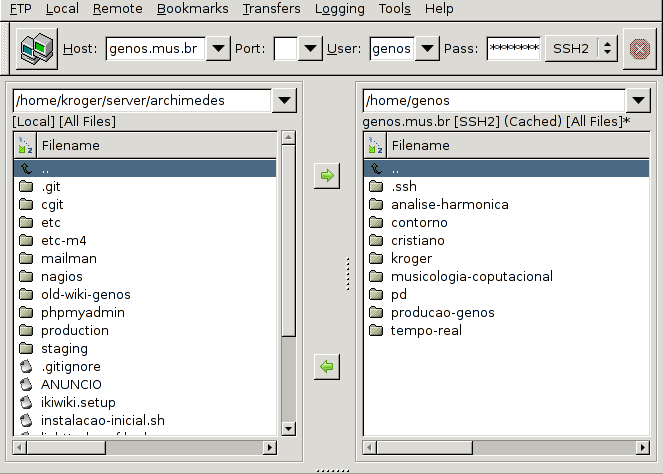
\includegraphics[scale=.7]{gftp-genos}
  \caption{Acessando repositório de arquivos com gftp}
  \label{fig:gftp}
\end{figure}


\chapter{Pesquisas do Genos}
\label{cha:pesquisas-do-genos}

A equipe multidisciplinar do Genos é formada por pesquisadores e
estudantes de graduação e pós-graduação da área de Música e Ciência da
Computação de diferentes instituições do Brasil. Diferentes pesquisas
são realizadas simultaneamente junto ao grupo. O líder do grupo
encabeça a pesquisa de análise harmônica (vide
\url{http://wiki.genos.mus.br/PesquisaGenos}), que demanda o maior
número de pessoas.

As principais pesquisas em execução no Genos atualmente são:

\begin{enumerate}
\item Análise harmônica automática.
\item Composição musical a partir de combinações de operações com
  contornos melódicos.
\item Estratégias de interação entre músico e computador através de
  Pure data.
\item Extração automática de motivos.
\item Po(i)ética em movimento: o movimento como propulsor de
  realidades composicionais
\end{enumerate}

\chapter{Pesquisa de Análise Harmônica Automática}
\label{cha:anal-harm-autom}

\section{Começando na pesquisa}
\label{sec:comec-na-pesq}

Para trabalhar em pesquisas do Genos é necessário garantir a
comunicação com o grupo, habituar-se às ferramentas utilizadas, e
executar prontamente as tarefas.

\subsection{Passo-a-passo de um novato no Genos}
\label{sec:passo-passo-de}

Os passos para um novato nas pesquisas do Genos são:

\begin{enumerate}
\item Associar-se às duas listas de discussão (vide capítulo
  \ref{cha:comunicacao}):
  \begin{enumerate}
  \item \url{http://lists.genos.mus.br/cgi-bin/mailman/listinfo/genos-users}
  \item \url{http://lists.genos.mus.br/cgi-bin/mailman/listinfo/genos-pesquisa}
  \end{enumerate}
\item Inscrever-se no \textit{bugtrac}: \url{http://genos.mus.br/bugs}
  (vide seção \ref{sec:gerenc-de-taref}).
\item Instalar as ferramentas utilizadas (vide seção
  \ref{sec:ferr-util-na}).
\item Ler os artigos referentes à pesquisa.
\item Aprender a executar as tarefas necessárias à pesquisa.
\end{enumerate}

\section{Ferramentas utilizadas na pesquisa de análise harmônica}
\label{sec:ferr-util-na}

As principais ferramentas utilizadas na pesquisa de análise harmônica
são:

\begin{enumerate}
\item Emacs (vide capítulo \ref{cha:emacs}),
\item Git (vide capítulo \ref{cha:git}),
\item \LaTeX (vide capítulo \ref{cha:latex}),
\item Lilypond (vide seção \ref{sec:lilypond}),
\item Inkscape \ref{cha:inkscape},
\item Gimp \ref{cha:gimp}.
\end{enumerate}

Não é obrigatório o uso do Linux, embora seja altamente encorajado.

\section{Tarefas principais da pesquisa de análise harmônica automática}
\label{sec:taref-princ-da}

O Genos está desenvolvendo o
Rameau\footnote{\url{http://wiki.genos.mus.br/Rameau}}, um software
para análise harmônica automática. Para um maior entendimento da
pesquisa vide
\url{http://wiki.genos.mus.br/AnaliseHarmonicaAutomatica}.

As principais tarefas desta pesquisa para músicos são a criação de
gabaritos e a correção de partituras.

\subsection{Criação de gabaritos}
\label{sec:criacao-de-gabaritos}

Uma das funcionalidades do Rameau é a comparação da análise de
algoritmos com análises feitas por humanos. Uma das tarefas para
músicas é a criação de gabaritos com as análises das peças para
possibilitar esta comparação.

Durante a atual fase da pesquisa os gabaritos criados armazenam apenas
os tipos de acordes, e não a função harmônica. A música é dividida em
segmentos, de forma que a cada mudança de nota (esta mudança pode
acontecer em qualquer voz), temos um novo segmento. A figura
\ref{fig:choral-rameau} traz um fragmento de coral analisado pelos
algoritmos (ES tree, EC Knn, etc). O gabarito deste fragmento é
escrito desta forma (vide a linha \eng{Answer}).

\begin{figure}
  \centering
  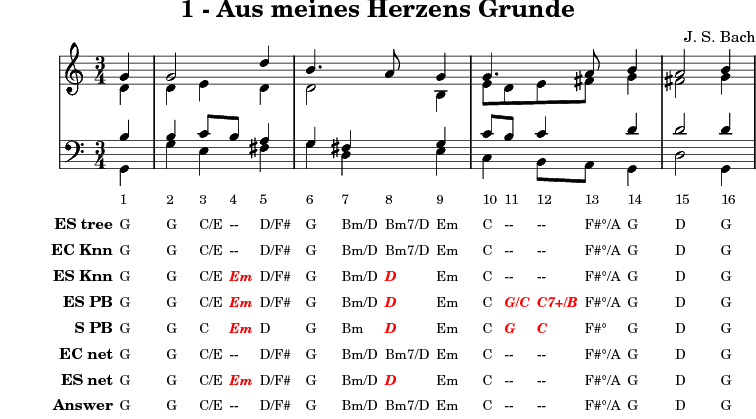
\includegraphics[scale=.8]{analysis-001}
  \caption{Coral analisado com o Rameau}
  \label{fig:choral-rameau}
\end{figure}

\begin{verbatim}
g
g c/e [b] d/f#
g bm/d bm7/d em
c [b d] [b] f#°/a g
d g
\end{verbatim}

\subsubsection{Formato de gabarito}
\label{sec:formato-de-gabarito}

As peças são cifradas em um formato .pop de acordo com o seguinte:

\begin{enumerate}
\item Cada segmento é identificado com uma cifra.
\item A duração de cada segmento é ignorada.
\item Cada linha do arquivo .pop deve conter apenas um compasso de
  cifras.
\item O espaçamento entre duas cifras é de um espaço.
\item Pausas são ignoradas e não são indicadas no gabarito.
\item Acordes são identificados com cifra comercial/popular:
  \begin{enumerate}
  \item Tríade maior é o padrão. Não precisa de complemento:
    \texttt{c}, \texttt{g};
  \item Tríade menor é indicada com $m$ após a tônica: \texttt{cm},
    \texttt{gm};
  \item Tríade diminuta leva $°$: \texttt{c°}, \texttt{d°};
  \item Tríade aumentada leva $+$: \texttt{c+}, \texttt{e+};
  \item Tétrades: todas levam obrigatoriamente um 7 no final:
    \begin{enumerate}
    \item menor com sétima: \texttt{cm7},
    \item menor com sétima maior: \texttt{cm7+},
    \item maior com sétima maior: \texttt{c7+},
    \item maior com sétima menor: \texttt{c7},
    \item diminuta: \texttt{c°7},
    \item semidiminuta: \texttt{cø7} (este caractere em geral fica nas
      teclas ``alt gr'' o),
    \item aumentada com sétima menor: \texttt{c+7}.
    \item aumentada com sétima maior: \texttt{c+7+}.
    \end{enumerate}
  \end{enumerate}
  \item Acidentes são $\#$ ou $b$: \texttt{c\#}, \texttt{bb}.
  \item Inversões são marcadas como \texttt{c/e}. Um arpejo no baixo
    teria uma cifra como \texttt{c c/e c/g c}.
\item Notas melódicas são identificadas com colchetes: \texttt{[d]},
  \texttt{[d f]} (duas notas melódicas simultâneas).
\item Acordes sem terça são identificados com ``!'': \texttt{c dm g7
    d g7 c d!  g7 c}. Os acordes que têm a terça subentendida pelo
  contexto não devem levar ``!''. Em um trecho em dó maior, por
  exemplo, se um acorde de sol sem terça está subentendido. No
  entanto, se ora esse acorde aparece maior, ora menor, pode não ser
  possível ter certeza. Então cifra-se \texttt{g!}.
\item Em caso de repetição de acordes em segmentos diferentes
  repete-se a cifra. Por exemplo: \texttt{c c dm g c c c c}.
\item Ritornelos são indicados com chaves. Por exemplo, \texttt{\{ c
    dm g c \}}.
\item Ambigüidades são indicadas em cada segmento com parênteses. Por
  exemplo: \texttt{c ([a] am) g}.
\item Em caso de cruzamento de vozes entre baixo e tenor, considera-se
  o tenor para definir a inversão do acorde.
\end{enumerate}

Um exemplo de gabarito pode ser visto em
\url{http://git.genos.mus.br/?p=rameau.git;a=blob;f=answer-sheets/chorales-bach/001.pop;h=1427035b706659afd0319e3dc7bccb0df1772283;hb=HEAD}

\subsubsection{Padrão de análise para gabaritos}
\label{sec:padrao-de-analise}

O Genos estabeleceu um padrão de análise para as cifras das
peças. Todos os gabaritos devem ser feitos de acordo com este
padrão. Exemplos podem ser vistos nos corais já analisados e
corrigidos (1 ao 25).

\begin{enumerate}
\item Acordes relativos em colcheias, em geral, são marcados como nota
  melódica.
\item Acordes que possuem acidentes, em geral, são entendidos a partir
  de alguma função secundária e são cifrados.
\item Um acorde de sétima deve ter esta nota resolvida
  descendentemente e por grau conjunto.
\item Um acorde de sétima que não seja de dominante deve ter sua
  sétima preparada pela mesma nota no acorde anterior.
\item Acordes aumentados ou de sexta aumentada não podem ser
  confundidos com segmentos com notas melódicas.
\end{enumerate}

\subsection{Correção de partituras}
\label{sec:corr-de-part}

As partituras utilizadas pela pesquisa são, em geral, convertidas de
um arquivo MIDI disponível livremente na internet, como por exemplo em
\url{http://www.jsbchorales.net/}, em um arquivo Lilypond (vide seção
\ref{sec:lilypond}). Entretanto, o resultado desta conversão pode
conter erros, principalmente porque o MIDI não armazena informações
enarmônicas. Por isso uma das tarefas dos músicos é conferir se o
arquivo convertido é equivalente à edição da partitura.

Para o corpus dos 371 corais da edição Riemenschneider há duas
maneiras de corrigir as partituras:
\begin{enumerate}
\item Comparando visualmente todas as notas da partitura gerada pelo
  Rameau com a edição Riemenschneider; ou
\item Ouvindo os nomes das notas geradas pelo Rameau e comparando com
  a edição Riemenschneider.
\end{enumerate}

\chapter{Comunicação}
\label{cha:comunicacao}

\section{Listas de discussão}
\label{sec:listas-de-discussao}

A comunicação entre os membros do Genos é feita através de duas listas
de discussão. A lista genos-users ---
\url{http://lists.genos.mus.br/cgi-bin/mailman/listinfo/genos-users}
--- é utilizada para todas as questões referentes ao uso do
laboratório, uso de ferramentas, e outros assuntos pertinentes ao
Genos. A lista genos-pesquisa ---
\url{http://lists.genos.mus.br/cgi-bin/mailman/listinfo/genos-pesquisa}
--- é utilizada para questões referentes à pesquisa de análise
harmônica, como decisões no desenvolvimento, dúvidas de funcionamento
do programa desenvolvido, e marcação de horários de reuniões.

Há ainda duas listas adicionais de mensagens automáticas. A lista
genos-commit ---
\url{http://lists.genos.mus.br/cgi-bin/mailman/listinfo/genos-commit}
--- é usada para a comunicação de alterações em todos os repositórios
do Genos. A lista genos-trac ---
\url{http://lists.genos.mus.br/cgi-bin/mailman/listinfo/genos-trac}
--- é utilizada para comunicar todas as tarefas gerenciadas pelo
\eng{bug trac}. É importante saber que estas listas \textbf{não
  recebem e-mails}.

\subsection{Escrevendo bons e-mails}
\label{sec:escrevendo-bons-e}

As listas de e-mails do Genos são úteis não apenas para comunicação no
tempo presente. Elas guardam históricos de dúvidas, dicas e soluções
de diversos assuntos. Por estes históricos serem constantemente
acessados, os e-mails devem ser organizados e bem escritos.

Para escrever ou responder e-mails de maneira produtiva, eficiente e
inteligente no Genos deve-se seguir estas regras:

\begin{enumerate}
\item Seja objetivo e sucinto no título. Se for possível fazer com que
  o leitor saiba o conteúdo do e-mail pelo título, faça acontecer. Por
  exemplo, se é preciso enviar um e-mail marcando horário de uma
  reunião de pesquisa, então faça um título como ``Reunião pesquisa em
  28/05 7:30''.
\item \textbf{NUNCA} misture assuntos diferentes em uma mesma
  mensagem. Se a mensagem é para marcar horário de reunião, não
  pergunte na mesma mensagem como instalar o Lilypond. Escreva outra
  mensagem com título ``Instalação do Lilypond'' e pergunte como
  instalar.
\item Seja objetivo e sucinto no corpo da mensagem. Fale apenas o que
  é necessário. Não precisa cumprimentar nem se despedir dos membros
  da lista. Apenas forneça a sua informação.
\item Não responda desnecessariamente. Se alguém informa que existe
  uma versão nova de um software, por exemplo, não responda para dizer
  ``legal'', ou ``OK''.
\item Se uma mensagem é mandada para propor horário de uma reunião
  responda sucintamente dizendo apenas ``posso'', ou ``não posso''. Se
  for uma reunião entre poucas pessoas, vale a pena colocar seus
  horários vagos.
\item Sempre que responder uma mensagem, \textbf{apague} o conteúdo
  da(s) mensagem(s) anteriores. Deixe apenas o que interessa. Veja
  exemplo mais abaixo. A lista naturalmente já guarda o histórico das
  mensagens de modo organizado. A repetição da mensagem apenas suja a
  lista.
\item Se você tem uma dúvida sobre o funcionamento de um programa,
  seja específico e dê informações para obter ajuda. Não diga apenas
  ``O programa dá um erro''. Copie parte do erro e cole na mensagem e
  fale em que circunstâncias ele ocorre.
\item Se alguém tirou sua dúvida, informe na lista que o seu problema
  foi resolvido, e, se possível, o que aconteceu. Isso ajudará muita
  gente que venha a ter o mesmo problema que você.
\item Preocupe-se em escrever bons e-mails, mas não perca seu tempo
  tentando escrever e-mails perfeitos. Seja apenas claro e
  objetivo. Use o tempo para escrever artigos e não e-mails.
\item Não use destaques desnecessários como escrever TUDO EM MAIÚSCULO
  ou fazer afirmações com muitas exclamações!!!!! Isso deixa a
  mensagem suja, concorda?????
\end{enumerate}

Abaixo um exemplo de e-mail de uma dúvida

\begin{verbatim}
Genos,

Quero rodar análise harmônica com o rameau. Rodei o comando

rameau analise -f 110

e obtive o erro:

unhandled SIMPLE-ERROR in thread #<SB-THREAD:THREAD "initial thread" {CFFFA01}>:
  expression should be in the format <substring>:<expression>

Marcos.
\end{verbatim}

A resposta de ajuda mantém a parte mais importante da mensagem
anterior e remove o resto. Observe:

\begin{verbatim}
Marcos escreveu:
> Quero rodar análise harmônica com o rameau. Rodei o comando
> 
> rameau analise -f 110

Faltou especificar o tipo de partitura:

rameau analise -f choral:110

Alexandre.
\end{verbatim}

E a informação de que a ajuda funcionou é sucinta:

\begin{verbatim}
Alexandre escreveu:
> Faltou especificar o tipo de partitura:
> 
> rameau analise -f choral:110

Ok, funcionou.

Marcos.
\end{verbatim}

\section{Reuniões}
\label{sec:reunioes}

Os membros do Genos se reunem para:

\begin{enumerate}
\item Discutir a pesquisa de análise harmônica

  As reuniões para a pesquisa de análise harmônica são semanais e têm
  o horário combinado a cada semestre. Para o semestre 2008.1 o
  horário oficial é sexta-feira, às 13 horas no GenosLab. Entretanto
  sempre é possível haver reuniões em outros horários e locais (como o
  Instituto de Matemática da UFBA).

  Durante a preparação de artigos, comunicações, ou palestras, as
  reuniões passam a ser mais freqüentes por causa da demanda de
  assuntos. Além das reuniões presenciais, eventualmente são
  realizadas reuniões virtuais por meio eletrônico, através do IRC
  (vide seção \ref{sec:reunioes-virtuais}).

\item Avaliar e planejar atividades

  As reuniões para planejamento e avaliação de atividades são
  combinadas entre os integrantes no final e início do semestre
  letivo, no GenosLab.

\end{enumerate}

Uma dica: seja pontual. Reuniões no Genos costumam acontecer na hora
marcada, e, dependendo da objetividade e demanda de assuntos, pode ser
muito rápida. O recorde via IRC foi uma reunião de seis minutos, e
presencialmente, de vinte minutos.

\subsection{Reuniões virtuais}
\label{sec:reunioes-virtuais}

%% FIXME: inserir tutorial de como configurar o IRC.
As esporádicas reuniões virtuais acontecem via IRC, no canal genos.

\section{Gerenciamento de tarefas}
\label{sec:gerenc-de-taref}

A comunicação das tarefas de cada membro do Genos é feita com o
\textit{bug trac}, um sistema online de gerenciamento de tarefas onde
todas as tarefas dos membros dos Genos são postadas. Através deste
sistema é possível acompanhar o andamento dos projetos do grupo a
partir das tarefas de cada membro. Este sistema está disponível em
\url{http://genos.mus.br/bugs}.

\subsection{Tutorial do sistema de gerenciamento de tarefas}
\label{sec:tutorial-do-sistema}

No \eng{bug trac} existem três conceitos
fundamentais. \texttt{Tickets} são tarefas a
executar. \texttt{Milestones} são objetivos no
tempo. \texttt{Components} são módulos do programa.

O uso do \eng{bug trac} consiste em:

\begin{enumerate}
\item Criar tarefas (tickets) para alguém realizar, podendo
  relacioná-las a versão do programa, milestonese e components.
\item Comunicar o encerramento das tarefas, ou seja, fechar os tickets
  das tarefas encerradas.
\end{enumerate}

Cada ticket tem um número único de identificação. Dessa forma é comum
se referir à tarefa pelo número do ticket.

\subsubsection{Menus do bug trac}
\label{sec:menus-do-bug}

O \eng{bug trac} tem três linhas de menu na parte superior direita.

Para registrar-se o usuário utiliza \eng{Register}, e para trabalhar o
usuário sempre deve se autenticar através do menu \eng{Login}.

O menu principal tem os seguintes links:

\begin{enumerate}
\item Wiki. Descreve o sistema e tem informações importantes como o
  calendário e o planejamento das versões do programa desenvolvido na
  pesquisa.
\item Timeline. Mostra em ordem cronológica todos os tickets criados,
  fechados, realocados e deixados sem fazer.
\item Roadmap. Mostra um mapeamento de execução de todos os
  milestones, informando quando cada milestone foi iniciado, quantos
  tickets cada um contém, e qual percentual de cada um já foi
  cumprido.
\item View Tickets. Mostra todos os tickets com vários filtros.
\item New Ticket. Abre um novo ticket, ou seja, cria uma nova tarefa.
\item Search. Procura por palavras em todos os tickets.
\end{enumerate}

\subsubsection{Criando tickets}
\label{sec:criando-tickets}

Para criar um ticket basta clicar em \eng{New Ticket}. Os campos
presentes são:

\begin{enumerate}
\item Short summary. É o título curto da tarefa. Por exemplo,
  ``Criar figuras com quintas paralelas''.
\item Type. Tipo de ticket. Pode ser uma tarefa, relato de bug,
  etc.
\item Full Description. Local para explicar detalhadamente, caso
  necessário, qual a tarefa e como executar. Por exemplo:
\begin{verbatim}
1. Rodar o comando
rameau parallel-fifths -f chora:001..371
2. Gerar partituras com análise dos corais com quintas paralelas:
rameau analise -f chora:001 -s
3. Gerar png das partituras:
lilypond --png music/chorales-bach/analysis-001.ly
4. Editar png: recortar o sistema onde acontecem as quintas e circulá-las.
\end{verbatim}
\item Priority. Prioridade do ticket.
\item Component. Módulo do programa. Por exemplo ``analise corais''.
\item Milestone. Objetivo no tempo. Por exemplo ``artigo anppom
  2008''.
\item Version. Versão do que está sendo feito. Por exemplo ``Rameau
  3.0''.
\item Assign to. É o dono do ticket. Pessoa que vai executar a
  tarefa. Por exemplo, ``Natanael''.
\end{enumerate}

Depois basta clicar em \eng{Submit ticket}.

São obrigatórios apenas os campos Short summary, type, component e
assign to.

Estes campos podem ser vistos na figura \ref{fig:trac-newticket}.

\begin{figure}
  \centering
  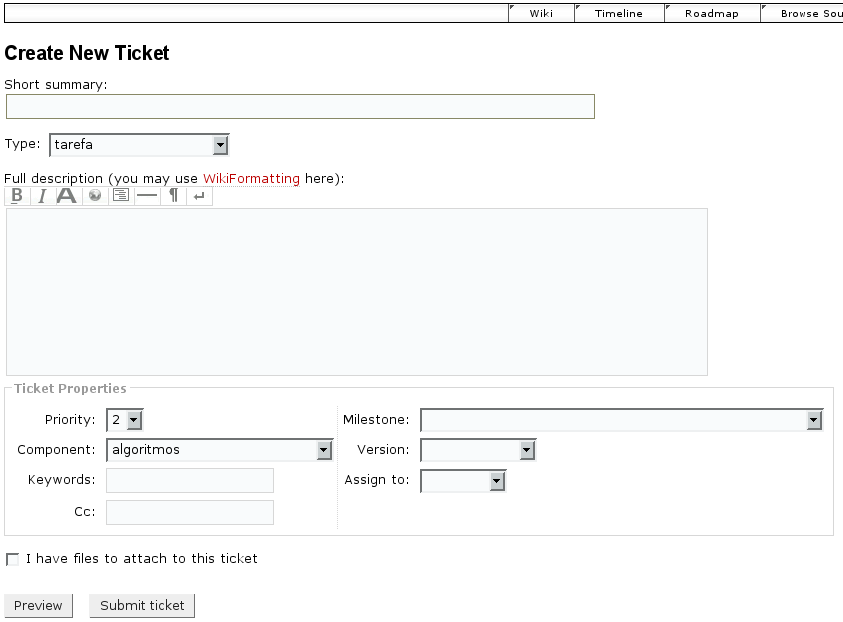
\includegraphics[scale=.7]{trac-newticket}
  \caption{Janela de criação de ticket no bug trac}
  \label{fig:trac-newticket}
\end{figure}

\subsubsection{Visualizando os tickets}
\label{sec:visu-os-tick}

É possível visualizar tickets de várias maneiras: ativos, fechados,
todos, os do usuário autenticado, separados por milestones, por donos,
etc. Cada uma dessas opções dá um relatório dos tickets com várias
informações.

\subsubsection{Fechando tickets}
\label{sec:fechando-tickets}

Para fechar um ticket é preciso encontrá-lo (vide seção
\ref{sec:visu-os-tick}) e então mudar a ação de \eng{leave as new}
para \eng{resolve}, escolher \eng{fixed} para fechar, e então clicar
em \eng{Submit changes}. Vide figura \ref{fig:trac-closeticket}.

\begin{figure}
  \centering
  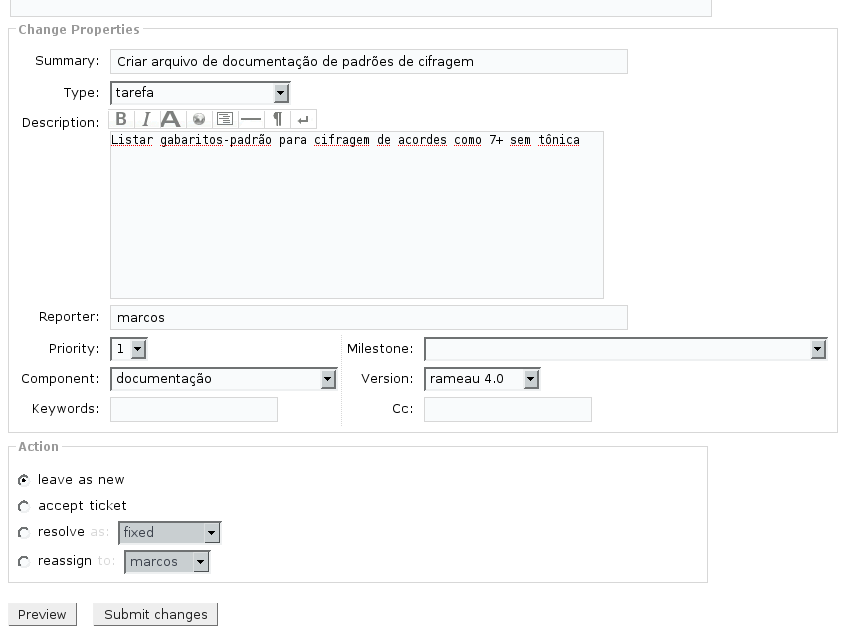
\includegraphics[scale=.7]{trac-closeticket}
  \caption{Janela de alteração de ticket no bug trac}
  \label{fig:trac-closeticket}
\end{figure}

\chapter{Uso do GenosLab}
\label{cha:uso-do-genoslab}

O laboratório GenosLab é administrado inteiramente pelo Genos. O seu
uso é restrito aos membros do grupo que estão desenvolvendo
pesquisa. Cada um desses membros tem direito a uma cota de uso do
laboratório. Os horários desta cota são acertados a cada semestre em
reunião geral do grupo, e pode ser negociado com prévio aviso na lista
genos-users.

O Genos tem três modalidades de uso normal:
\begin{enumerate}
\item Para gravação (uso exclusivo e individual de um membro)
\item Para mixagem com som externo (uso compartilhado)
\item Para uso comum com uso obrigatório de headphones (uso
  compartilhado)
\end{enumerate}

Na modalidade ``comum'' é possível haver reunião e orientação no
laboratório.

A prioridade dos horários do GenosLab é dedicada aos cursos do Genos.

Os horários de uso ficam disponíveis em
\url{http://wiki.genos.mus.br/HorariosGenoslab}

\section{Segurança do GenosLab}
\label{sec:segur-do-genosl}

Estas são informações para manter a segurança do equipamento do
GenosLab:

\begin{enumerate}
\item \underline{\textbf{Nunca}} deixe a porta destrancada com a sala
  vazia. Se for sair além da escada de acesso tranque a porta.
\item Nunca deixe um desconhecido sozinho no GenosLab. Entenda por
  desconhecido qualquer um que não faça parte da equipe Genos.
\item Ao fim do trabalho, ao sair do GenosLab confira se os
  computadores, o Furmann e o ar condicionado estão desligados, se os
  armários estão devidamente trancados, e apague as lâmpadas interna e
  externa.
\item Caso tenha usado microfones, headphones ou quaisquer
  equipamentos que fiquem guardados em armários, coloquem de volta no
  lugar antes de sair.
\end{enumerate}

\section{Equipamento}
\label{sec:equipamento}

O equipamento não poderá sair do laboratório. \textbf{Apenas o
  coordenador do laboratório poderá emprestar equipamento}, ainda
assim documentando através da lista de discussão.

\chapter{Coordenação do GenosLab}
\label{cha:coordenacao-do-genos}

As principais tarefas do coordenador do GenosLab são

\begin{itemize}
\item Manter as máquinas funcionando permanentemente
\item Marcar reuniões semestrais para:
  \begin{itemize}
  \item marcar horários de uso do estúdio
  \item planejar cronograma dos cursos de extensão
  \item providenciar manutenção de equipamentos
  \end{itemize}
\end{itemize}

\part{Ferramentas}
\label{part:ferramentas}

\chapter{Instalando e configurando o Arch}
\label{cha:inst-e-conf}

To get it up and running change the /etc/man.conf file and change the PAGER and BROWSER variable to:

PAGER           /usr/bin/most -s
BROWSER         /usr/bin/most -s

\chapter{Repositórios debian}
\label{cha:repositorios-debian}

Para instalar o csound5 você deve usar o pacote debian do Genos. Para
isso coloque a seguinte linha no seu \texttt{/etc/apt/sources.list}
(como root):

\begin{verbatim}
deb http://genos.mus.br/ debian/
\end{verbatim}

Em seguida rode o comando

\begin{verbatim}
aptitude update
\end{verbatim}

Agora você pode instalar os programas disponíveis no genos digitando
algo como o comando abaixo como root.

\begin{verbatim}
aptitude install <nome do programa>
\end{verbatim}

\section{Debian}
\label{sec:debian}

\section{Modo emacs para apt}
\label{sec:modo-emacs-para}

http://www.netfort.gr.jp/~dancer/software/apt-mode.html

\chapter{Git}
\label{cha:git}

\section{Introdução}
\label{sec:introducao}

O Git (o ``g'' é pronunciado como na palavra gato e não como ``jit'')
é um programa para controle de versão distribuído desenvolvido por
Linus Torvalds (o criador do Linux) e mantido por Junio C Hamano. A
página do git em \url{http://git.or.cz/} tem vários tutoriais e
manuais.

\section{Instalação}
\label{sec:instalacao-3}

Para instalar o git no debian execute o seguinte comando.

\begin{verbatim}
aptitude install git-core git-completion git-doc git-gui gitk ssh
\end{verbatim}

É uma boa idéia configurar o git para usar o seu nome e email:

\begin{verbatim}
git config --global user.name "Seu Nome"
git config --global user.email "seu@email.com.br"
\end{verbatim}

\section{Repositórios do genos}
\label{sec:acesso-de-escrita}

O genos mantém diversos repositórios listados em
\url{git.genos.mus.br}. Para ter acesso de escrita você precisa criar
uma chave pública de criptografia. Para isso rode o comando:

\begin{verbatim}
ssh-keygen -t rsa
\end{verbatim}

Esse comando vai fazer uma série de perguntas como o tamanho da chave,
seu nome e email, etc. Se você não souber a resposta para alguma
pergunta não precisa se preocupar, o valor padrão deve ser o
suficiente. Quando ele pedir uma passphrase, certifique-se que você
não vai esquecê-la! A chave pública vai ser geradad no arquivo
\texttt{~/.ssh/id\_rsa.pub}. Para ter acesso de escrita nos
repositórios do genos envie o arquivo para Pedro Kroger. Para saber
mais sobre geração de chaves, veja
\url{http://kimmo.suominen.com/docs/ssh/}.

Se você enviou a chave pública e seu acesso foi liberado, você pode
baixar um projeto no repositório do genos com o comando abaixo:

\begin{verbatim}
git clone ssh://cons@genos.mus.br/repos/<nome do projeto>
\end{verbatim}

Por exemplo, para baixar o projeto rameau você deve
digitar:

\begin{verbatim}
git clone ssh://cons@genos.mus.br/repos/rameau.git
\end{verbatim}

Contudo, se você não tem acesso de escrita ao repositório, ou seja,
não tem permissão para modificar o repositório diretamente, você ainda
pode baixar um projeto e contribuir mudanças (veja a seção
\ref{sec:enviando-patches}). Para isso baixe o repositório com o
comando abaixo:
$\langle 4 \: 3\:  2\: 1 \rangle$
\begin{verbatim}
git clone git://genos.mus.br/<nome de repositório>
\end{verbatim}

\section{Comandos básicos}
\label{sec:comandos-basicos}

Para gravar uma mudança é necessário primeiro adicioná-la ao
index. Modifique alguns arquivos e então adicione seu conteúdo
atualizado ao index:

\begin{verbatim}
git add arquivo1 arquivo2 arquivo3
\end{verbatim}

Para ver um sumário da situação do repositório utilize:

\begin{verbatim}
git status
\end{verbatim}

Você então deve gravar suas mudanças com:

\begin{verbatim}
git commit -m "mensagem descrevendo o commit"
\end{verbatim}

Caso queira adicionar todos os arquivos modificados pode fazer:

\begin{verbatim}
git commit -a -m "mensagem descrevendo o commit"
\end{verbatim}

Use o comando abaixo para enviar suas mudanças para o repositório
central:

\begin{verbatim}
git push
\end{verbatim}

Para atualizar sua cópia local, ou seja, para baixar as mudanças que
outros tenham feito no repositório, use os comandos:

\begin{verbatim}
git pull --rebase
\end{verbatim}

onde <branch remoto> é o branch remoto onde o desenvolvimento
acontece. Provavelmente é master.

Para reverter as mudanças que não foram enviadas use

\begin{verbatim}
git checkout -f
\end{verbatim}


\section{Pull vs Rebase}

Existem dois jeitos de importar as mudanças de um repositório remoto
pro repositório local. Elas são o ``pull'' e o ``rebase''. A diferença
é a forma como as mudanças locais são mantidas na hora de importar as
remotas.

Imagine uma árvore de commits assim (onde local é o branch atual de desenvolvimento):

\begin{verbatim}
                     A---B---C local
                    /
               D---E---F---G master
\end{verbatim}

Após um ``git pull'' aplicado no computador local, a árvore fica:

\begin{verbatim}
                     A---B---C---F'--G' local
                    /           /
               D---E---F---G ----master
\end{verbatim}

Após um git push, a árvore no repositório remoto fica

\begin{verbatim}
                     A---B---C---F'--G'-- 
                    /           /        \
               D---E---F---G -------------A'--B'--C'--F''--G''  master
\end{verbatim}

Isso não é muito interessante por serem feitos, ao todo, dois merges
das mudanças locais no repositório remoto. Com mais de duas pessoas
fazendo mudanças ao mesmo tempo esse método gera árvores de histórico
complicadas e difíceis de entender depois, com vários merges.

Uma alternativa é usar ``git pull -\,-rebase'' em vez de ``git
pull''. Fazendo isso, a árvore local, que era

\begin{verbatim}
                     A---B---C local
                    /
               D---E---F---G master
\end{verbatim}

fica

\begin{verbatim}
                             A'---B'---C' local
                            /
               D---E---F---G master
\end{verbatim}

Após um ``git push'', a árvore do servidor fica

\begin{verbatim}
                             A'---B'---C'-
                            /             \
               D---E---F---G ---------------  master
\end{verbatim}

ou

\begin{verbatim}
               D---E---F---G---A'--B'--C'-----  master
\end{verbatim}

o que é muito mais limpo. Mesmo com várias pessoas desenvolvendo isso
tende a gerar históricos mais lineares.

\section{Escrevendo boas mensagens de commit}
\label{sec:escr-boas-mens}

Além de usar a opção \texttt{-m} para indicar a mensagem de commit,
você também pode digitar apenas \texttt{git commit} onde o git vai
abrir o editor padrão para você digitar a mensagem de commit. Em geral
o editor padrão é o vi. Eu sugiro que você coloque a linha abaixo no
seu \texttt{~/.bashrc}:

\begin{verbatim}
  export EDITOR="emacs"
\end{verbatim}

Desse modo o git sempre vai abrir o emacs para pedir a mensagem de
commit.

Em geral uma mensagem de commit tem o seguinte formato:

\begin{verbatim}
primeira linha

texto mais longo texto mais longo texto mais longo
texto mais longo texto mais longo texto mais longo
texto mais longo texto mais longo texto mais longo 
\end{verbatim}

Onde a primeira linha é um breve sumário da modificações, o texto mais
longo contém mais detalhes. Observe que elas são separadas por uma
linha em branco.

\section{Usando diferentes ramos}
\label{sec:usando-o-git}

Para ver os ramos do repositório basta usar o comando

\begin{verbatim}
git branch
\end{verbatim}

Para mudar de ramo usa-se o comando

\begin{verbatim}
git checkout
\end{verbatim}

Mudando do ramo master para novo-ramo:

\begin{verbatim}
git checkout novo-ramo
\end{verbatim}

Conferindo o novo ramo:

\begin{verbatim}
git branch
  master
* novo-ramo
\end{verbatim}

Para criar um novo ramo e mudar para ele automaticamente usa-se

\begin{verbatim}
git checkout -b novo-ramo
\end{verbatim}

Para ver a lista de commits no novo-ramo em relação a master (pode-se
usar a opção \texttt{-p} para ver um diff do código:

\begin{verbatim}
git log  master..novo-ramo
\end{verbatim}

Para enviar um novo ramo para o repositório remoto:

\begin{verbatim}
git push origin ramo-local:ramo-remoto
\end{verbatim}

Talvez você tenha que usar o caminho completo para o ramo, como em:

\begin{verbatim}
git push origin refs/heads/ramo-local:refs/heads/ramo-remoto
\end{verbatim}

Para listar os ramos em um repositório remoto

\begin{verbatim}
git branch -r
\end{verbatim}

Para apagar um ramo remoto:

\begin{verbatim}
git push origin :refs/heads/<ramo remoto>
\end{verbatim}

Para baixar um ramo no repositório remoto usa-se \texttt{git branch}
com a opção \texttt{--track}, indicando qual o nome do ramo local e o
nome do ramo remoto. É uma boa prática ter o mesmo nome para os ramos
local e remoto.

\begin{verbatim}
git branch --track novo-ramo origin/novo-ramo
\end{verbatim}

O nome \texttt{origin} nada mais é que um alias para a localização de
um repositório. Essa informação fica armazenada no arquivo
\texttt{.git/config} dentro do repositório. O trecho do
\texttt{.git/config} referente a configuração de \texttt{origin} pode
ser vista abaixo:

\begin{verbatim}
[remote "origin"]
        url = ssh://cons@genos.mus.br/repos/teste.git
        fetch = +refs/heads/*:refs/remotes/origin/*
\end{verbatim}

Veja na seção \ref{sec:o-arquivo-config} outras possibilidades de uso
para o arquivo \texttt{.git/config}.

Para manter os ramos atualizados, \texttt{git pull} e \texttt{git
  push} devem ser suficientes. O Git mantém cada ramo separado sem
interferir no outro. Contudo, mudanças sem commit vão aparecer em
todos os ramos.

Para mesclar as mudanças do branch \texttt{master} no seu ramo é só
fazer:

\begin{verbatim}
git pull .
\end{verbatim}

\section{Escolhendo commits específicos (cherry picking)}
\label{sec:escolh-comm-espec}

Você pode aplicar um commit específico na sua árvore com
\texttt{cherry-pick}. No exemplo abaixo estamos no branch master e o
commit 85cd08ee1aec0fbd3cf3d696a70872639e59212f aconteceu no branch
novo-ramo. Ele vai aplicar apenas esse commit em master.

\begin{verbatim}
git cherry-pick 85cd08ee1aec0fbd3cf3d696a70872639e59212f
\end{verbatim}

Isso é útil quando você corrigiu um bug em um ramo de desenvolvimento
e quer replica-lo no ramo principal.

\section{Resolvendo conflitos}
\label{sec:resolvendo-conflitos}

Quando um merge não é resolvido automaticamente pelo git ele indica
isso claramente. Você não vai conseguir dar um commit. Tanto commit
quanto status vão mostrar os arquivos que precisam resolver os
conflitos:

\begin{verbatim}
git commit
file.txt: needs merge
\end{verbatim}

Git vai marcar os conflitos no arquivo usando marcadores de conflito.
Abaixo podemos ver um conflito marcado com duas versões:

\begin{verbatim}
<<<<<<< variant A
Uma versão
>>>>>>> variant B
Outra versão
======= end
\end{verbatim}

Tudo que você precisa fazer é editar o arquivo para resolver os
conflitos e dar um commit com:

\begin{verbatim}
git add file.txt
git commit
\end{verbatim}

Se você usa emacs pode usar o \texttt{M-x vc-resolve-conflicts} para
lhe auxiliar na resolução de conflitos (ele funciona como o ediff).

\section{Revisões antigas}
\label{sec:revisoes-antigas}

Você pode ver uma versão antiga de um arquivo com \texttt{cat-file}:

\begin{verbatim}
git cat-file -p tags/v1.4.3:git.c
git cat-file -p f5f75c652b9c2347522159a87297820103e593e4:git.c
\end{verbatim}

\section{Enviando patches}
\label{sec:enviando-patches}

Para criar patches com suas modificações você deve usar o
\texttt{format-patch}. Esse comando vai gerar uma série de arquivos
numerados, como \texttt{0001-mais-stuff.patch}. Você deve enviar esses
arquivos para a lista de discussão apropriada.

\begin{verbatim}
 git format-patch origin/master
\end{verbatim}

Se a quantidade de patches for muito grande, você pode usar o
\texttt{git-send-email}, caso contrário é ok usar seu cliente de email
favorito.

\section{Configuração}
\label{sec:configuracao}

\subsection{Usando abreviações}
\label{sec:usando-abreviacoes}

Eu sugiro que você coloque algo como a linha abaixo no seu
\texttt{~/.bashrc}.

\begin{verbatim}
export repos=ssh://cons@genos.mus.br/repos
\end{verbatim}

Desse modo você poderá baixar um projeto de uma maneira mais fácil:

\begin{verbatim}
git clone $repos/rameau.git
\end{verbatim}

\subsection{O arquivo config}
\label{sec:o-arquivo-config}

Você pode configurar o arquivo \texttt{.git/config} de um repositório
local para usar nomes abreviados. Isso é particularmente útil se está
usando mais de um repositório ou ramos diferentes.

\begin{verbatim}
cat >>.git/config <<EOF
[remote "public-repo"]
        url = ssh://yourserver.com/~you/proj.git
EOF
\end{verbatim}

Você pode fazer a mesma coisa com \texttt{git remote}:

\begin{verbatim}
git remote add public-repo ssh://example.com/project.git
\end{verbatim}

\subsection{Saída colorida}
\label{sec:saida-colorida}

Se você é viciado em saída colorida vai querer executar os comandos abaixo:

\begin{verbatim}
git config --global color.diff auto
git config --global color.status auto
git config --global color.branch auto
\end{verbatim}

\section{Repositórios remotos}
\label{sec:remote}


O git tem um modo interno muito inteligente para lidar com
repositórios remotos. Cada repositório pode guardar ``ponteiros'' para
outros repositórios (chamados de \texttt{remotes} na documentação), e
o git tem comandos simples para enviar e receber ramos (``branches'')
desses repositórios. Como o git é bem flexível, vale a pena descrever
alguns fluxos de trabalho.

\subsection{Exportando um repositório local}
\label{sec:export-local}

Às vezes se começa a trabalhar em um repositório, se faz coisas e se
quer pegar essas coisas, colocar em um repositório remoto e manter os
dois atualizados.

A primeira coisa a se fazer nesse caso é criar o repositório
remoto. Para fazer isso, vá ao lugar remoto onde vai ficar o
repositório, crie um diretório com o nome desejado, vá para esse
diretório e execute
\begin{verbatim}
$ git init
\end{verbatim}
Isso vai inicializar um repositório git vazio no lugar escolhido.

Depois, vá para o seu repositório local e execute
\begin{verbatim}
$ git remote add <nome-remoto> <caminho-para-o-repo-remoto>
$ git push <nome-remoto> refs/heads/master:refs/heads/master
\end{verbatim}
onde <nome-remoto> é o nome que você deseja dar para o repositório
remoto (o nome padrão pra isso é \texttt{origin}) e
<caminho-para-o-repo-remoto> é o caminho onde foi colocado o outro
repo. Se ele é local, basta um ../foo/bar, se ele está num servidor
com suporte ao protocolo git o endereço é parecido com
\texttt{git://servidor/repo.git}, e se ele está num servidor com ssh o
caminho é algo como \texttt{ssh://usuario@servidor/caminho/repo.git}.

Depois desses comandos um
\begin{verbatim}
$ git pull <nome-remoto>
\end{verbatim}
faz o pull das modificações no repo remoto.

\subsection{Clonando um repositório remoto}
\label{sec:clone}

O procedimento para clonar um repo remoto está descrito na seção
\ref{sec:acesso-de-escrita}.

\chapter{Gravação de CD e DVD}
\label{cha:gravacao-de-cd}

\section{Copiando um CD ou DVD}
\label{sec:copiando-um-cd}

A maneira mais fácil de copiar um DVD ou CD completamente é usando o
\texttt{dd}. A opção \texttt{if} (\textit{input file}) indica o
dispositivo do DVD ou CD e a opção \texttt{of} (\texttt{output file})
indica o nome da imagem que será gerada:

\begin{verbatim}
dd if=/dev/sr1 of=arquivo.iso
\end{verbatim}

O arquivo gerado será uma réplica exata do CD. Inclusive você pode
montar a imagem usando mount:

\begin{verbatim}
mount -o loop /tmp/arquivo.iso /mnt
\end{verbatim}

\section{Identificando o fabricante da mídia}
\label{sec:ident-o-fabr}

Para identificar o verdadeiro fabricante de uma mídia de DVD use o
comando \texttt{dvd+rw-mediainfo} como abaixo:

\begin{verbatim}
dvd+rw-mediainfo /dev/dvd
\end{verbatim}

Para identificar o verdadeiro fabricante de uma mídia de CD use a
opção \texttt{-atip} do wodim.

\begin{verbatim}
wodim -atip 
\end{verbatim}

\section{Recuperando dados}
\label{sec:recuperando-dados}

Se o disco tem problemas o \texttt{ddrescue} pode ser uma boa opção.
Para ler um disco:

\begin{verbatim}
ddrescue /dev/dvd DVD.iso DVD.log
\end{verbatim}

Se \texttt{ddrescue} reportar algum erro, tente uma segunda vez com o
acesso direto ao disco ativado:

\begin{verbatim}
ddrescue -d -r1 /dev/dvd DVD.iso DVD.log
\end{verbatim}

\chapter{Emacs}
\label{cha:emacs}

Emacs é o melhor editor de texto que eu já encontrei na vida. É um
editor altamente customizável, capaz de reconhecer diversos formatos e
fornecer ferramentas para lidar com diversas sintaxes. Possui inúmeros
pacotes que o permitem funcionar como leitor de e-mails, navegador de
internet, cliente de mensagem instantânea, gerenciador de arquivos,
gerenciador de bibliografia, planilha eletrônica, calculadora
científica, visualizador de imagens e psicoterapeuta (isso mesmo!).

O site oficial é \url{http://www.gnu.org/software/emacs/}, e as
ferramentas podem ser vistas em: \url{http://www.emacswiki.org/}. Um
guia rápido para as teclas pode ser visto em
\url{http://ccrma.stanford.edu/guides/package/emacs/emacs.html}.

\section{Instalação}
\label{sec:instalacao-7}

\subsection{Linux}
\label{sec:linux}

Há 3 formas de instalar o Emacs no Linux:

\begin{enumerate}
\item Usando um pacote disponível na distribuição
\item Rodando um binário disponível pelo projeto
\item Compilando a versão de desenvolvimento do repositório do projeto
\end{enumerate}

Na instalação através de um pacote usa-se, no Debian:

\begin{verbatim}
sudo apt-get update
sudo apt-get install emacs
\end{verbatim}

E no ArchLinux:

\begin{verbatim}
pacman -Sy emacs
\end{verbatim}

Para instalar por um binário é preciso baixá-lo em
\url{http://ftp.gnu.org/pub/gnu/emacs/}, descompactá-lo e instalá-lo.

Para compilar a versão de desenvolvimento é preciso usar o
cvs. Maiores instruções em:
\url{http://savannah.gnu.org/cvs/?group=emacs}

\subsection{Windows}
\label{sec:windows}

O Emacs é instalado no Windows através de um binário como
\texttt{emacs-22.2-bin-i386.zip} disponível em:
\url{http://ftp.gnu.org/pub/gnu/emacs/windows/}

\section{Configuração do Emacs}
\label{sec:conf-do-emacs}

O Emacs carrega o arquivo de configuração \verb!.emacs!. Este arquivo
deve ser colocado na pasta pessoal do usuário. No Linux ele fica em
\verb!/home/usuario/.emacs!. Para saber qual a pasta correta abra o
Emacs, digite o comando \verb!(insert (getenv "HOME"))! e compute com
C-x C-e.

\subsection{Ponto emacs básico}
\label{sec:dot-emacs-basico}

\begin{verbatim}
(put 'upcase-region 'disabled nil)
(put 'narrow-to-region 'disabled nil)
(put 'downcase-region 'disabled nil)
(put 'overwrite-mode 'disabled t)

(setq display-time-day-and-date t
      display-time-24hr-format t
      confirm-kill-emacs 'yes-or-no-p
      inhibit-startup-message t
      font-lock-maximum-decoration t
      sentence-end-double-space nil ; usa espaços simples para sentenças
      default-abbrev-mode t
      vc-follow-symlinks t
      x-select-enable-clipboard t
      text-mode-hook '(turn-on-auto-fill footnote-mode text-mode-hook-identify)
      ediff-window-setup-function 'ediff-setup-windows-plain
      ediff-split-window-function 'split-window-horizontally)

(setq-default indent-tabs-mode nil)
(tool-bar-mode -1)
(show-paren-mode t)
(display-time-mode t)
(column-number-mode t)
(ido-mode t)
(transient-mark-mode -1)

(fset 'yes-or-no-p 'y-or-n-p) 
(set-default-coding-systems 'utf-8)

;; descomente isso para salvar todos os backups em um unico lugar
;;(setq backup-by-copying t
;;      backup-directory-alist '(("." . "~/tmp/emacs-backups"))
;;      delete-old-versions t
;;      kept-new-versions 6
;;      kept-old-versions 2
;;      version-control t)

;;; replace string
(global-set-key (kbd "C-c r") 'replace-string)

;;; footnote mode
(autoload 'footnote-mode "footnote" nil t)
(add-hook 'message-mode-hook 'footnote-mode)
(add-hook 'text-mode-hook 'footnote-mode)

;;; git (vc-mode)
(when (featurep 'vc-git)
  (add-to-list 'vc-handled-backends 'git))

;;; erc
(eval-after-load "erc"
  '(progn
     ;(easy-menu-add-item  nil '("tools") ["IRC" erc-select t])
     (setq erc-timestamp-format "[%H:%M] ")
     (erc-autojoin-mode 1)
     (setq erc-autojoin-channels-alist
     '(("freenode.net" "#lisp" )))))

;;; ispell
(eval-after-load "ispell"
  (progn
    (setq ispell-silently-savep t
    ispell-program-name "aspell"
    ispell-dictionary "american")))

;;; nxml
(add-to-list 'auto-mode-alist
       (cons (concat "\\." (regexp-opt '("xml" "xsd" "sch" "rng" "xslt" "svg" "rss") t) "\\'")
       'nxml-mode))
(unify-8859-on-decoding-mode)
(setq magic-mode-alist
      (cons '("<\\?xml " . nxml-mode)
      magic-mode-alist))
(fset 'xml-mode 'nxml-mode)
\end{verbatim}

\section{Definir teclas}
\label{sec:teclas}

Para definir uma tecla de atalho no seu \texttt{.emacs}, use algo como

\begin{verbatim}
(global-set-key [(foo bar) baz]  'funcao-a-ser-executada)
\end{verbatim}

Para definir teclas em um modo específico,

\begin{verbatim}
(define-key slime-mode-map [(alt control u)] 'rameau-cria-teste-defun)
(define-key slime-mode-map [(control return)] 'rameau-new-test)
\end{verbatim}

\section{Macros}
\label{sec:macros}

Macros de teclado são simples de usar. \texttt{C-x (} começa a gravar
uma macro e \texttt{C-x )} termina. Para executar, \texttt{C-x
  e}. Macros aceitam um comando de prefixo, com \texttt{C-x u
  <<numero>>} antes do \texttt{C-x e}. Para perguntar se o usuário
quer continuar, use \texttt{C-x q} durante a gravação da macro. Para
dar nome à macro, \texttt{M-x name-last-kbd-macro}. \texttt{M-x
  insert-kbd-macro} insere a definição de uma macro no buffer atual,
útil pra guardar no .emacs. Para editar uma macro, \texttt{C-x k RET},
e \texttt{C-c C-c} para terminar a edição.

\section{Snippet}
\label{sec:snippet}

\texttt{snippet.el} (disponível em
\url{http://www.kazmier.com/computer/snippet.el} é uma biblioteca
genial para inserir templates de texto. Um exemplo de uso é

\begin{verbatim}
(defun insert-texttt ()
  (interactive)
  (snippet-insert "\\\\texttt{$$}"))

(define-key LaTeX-mode-map [(meta control c)] 'insert-texttt)

\end{verbatim}

que cria a função \texttt{insert-texttt} no modo latex presa às teclas
\texttt{C-M-c}. Eu recomendo algo como

\begin{verbatim}
(define-key snippet-map [(control tab)] 'snippet-next-field)
(define-key snippet-map [(control shift tab)] 'snippet-prev-field)
\end{verbatim}

no \texttt{.emacs} para usar teclas para snippet.

\section{Dired}
\label{sec:dired}

Dired é o navegador de arquivos do Emacs. Ele é equivalente ao
Nautilus do gnome, Konqueror no KDE ou o Windows Explorer. As
vantagens principais do dired são integração com o Emacs,
automatização de operações em arquivos e velocidade de edição.

Para iniciar o dired, basta abrir um diretório com \texttt{C-x C-f} ou
então apertar \texttt{C-x d} ou digitar \texttt{M-x dired}.

A coisa mais simples de se fazer com o dired é deletar arquivos. Para
fazer isso, coloque o cursor em cima do arquivo a ser deletado e aperte
\texttt{d} para marcar o arquivo para remoção. Você pode marcar
quantos arquivos quiser. Depois, aperte \texttt{x} para executar a
deleção. \texttt{g} atualiza a tela do dired. Para desmarcar um
arquivo, use \texttt{u}.

O dired também tem comandos para marcar automaticamente alguns
tipos de arquivos para deleção. \texttt{$\sharp$} marca os arquivos de
autosave, e \texttt{\~} marca os arquivos temporários. \texttt{\&}
sugere arquivos temporários para remoção. \texttt{\% d} permite que você
digite uma expressão regular e marca todos os arquivos que satisfaçam
essa expressão.

Para abrir um arquivo no dired, \texttt{RET} ou \texttt{f} dão conta
do recado. Para copiar, use \texttt{C} (C maiúsculo, não
control). Para renomear, \texttt{R}, para mudar as permissões
\texttt{M} e \texttt{Z} para gzipar o arquivo. \texttt{L} carrega o
arquivo no emacs (equivalente a \texttt{M-x load-file}). \texttt{A}
faz uma busca no arquivo e \texttt{Q} faz um replace. Dentro desses
comandos, \texttt{M-,} continua a operação. \texttt{!} roda um comando
do shell no arquivo. \texttt{\% u} e \texttt{\% l} renomeiam arquivos
para maiúsculas e minúsculas, respectivamente. \texttt{w} copia o nome
do arquivo selecionado para o clipboard.

Todas essas operações de arquivo operam ou em um arquivo ou em todos
os arquivos marcados. Para marcar um arquivo use \texttt{m} ou
\texttt{*}, e para marcar vários use \texttt{\% m}.

Para fazer um diff, selecione um arquivo com \texttt{C-SPC}, mova o
cursor até o outro arquivo e aperte \texttt{=}. \texttt{C-u i} insere
os conteúdos do subdiretório selecionado no buffer atual. \texttt{+}
cria um diretório.

Para entrar no modo editor, use \texttt{M-x
  wdired-change-to-wdired-mode}. Para salvar e sair, use \texttt{C-c
  C-c} e para sair sem salvar use \texttt{C-ESC}. Com uma linha tipo
\texttt{(setq wdired-allow-to-change-permissions t)} no
\texttt{.emacs} é possível editar as permissões dos arquivos.

\texttt{M-x image-dired} é uma versão do dired que mostra miniaturas
das imagens em um diretório.

\section{imenu}
\label{sec:imenu}

\texttt{imenu} é um modo útil do emacs para navegar dentro de um
arquivo de texto grande. Executar \texttt{imenu-add-menubar-index}
calcula um índice do arquivo separando as seções mais importantes, e
\texttt{M-x imenu} pede o nome de uma seção e pula para
ela. \texttt{imenu} funciona em praticamente qualquer modo do emacs.

No seu \texttt{.emacs} você pode colocar as linhas
\begin{verbatim}

(add-hook 'LaTeX-mode-hook 'imenu-add-menubar-index)
(define-key LaTeX-mode-map [(control meta g)] 'imenu)

\end{verbatim}
para habilitar o uso do \texttt{imenu} dentro do auctex, ativando-o
com \texttt{C-M-g}.

\section{Emacs-git}
\label{sec:emacs-git}

O \texttt{Emacs-Git} é um módulo para manipulação do controle de
versão \texttt{git} através do \texttt{Emacs}.

É possível baixar pelo repositório git:

\begin{verbatim}
git clone git://github.com/tsgates/git-emacs.git
\end{verbatim}

Para instalá-lo é necessário colocar estes arquivos no path do Emacs:

\begin{verbatim}
git-emacs.el
git-modeline.el
git-blame.el
\end{verbatim}

No \texttt{.emacs} é necessário colocar o caminho para estes arquivos
e requisitar o \texttt{git-emacs}:
\begin{verbatim}
(add-to-list 'load-path "/home/tsgates/Skills/git/git-emacs-1.0")
(require 'git-emacs)
\end{verbatim}

É possível usá-lo com M-x ou com teclas de atalho. Os comandos para o
M-x começam com git (eg. \texttt{M-x git-status}), e os atalhos
começam com C-x v (eg. \texttt{C-x v =} para git-status).

\section{Version Control (vc)}
\label{sec:vc}

vc provê uma interface uniforme de controle de versão para o Emacs. Funciona
com os principais controles de versão, tais como: git, svn e cvs. Para o
git é necessário instalar o vc-git.

Comando geral do vc, qualquer comando do vc inicia com essas teclas.
\begin{verbatim}                                                   
C-x v 
\end{verbatim}

Marca o arquivo para controle de versão
\begin{verbatim}                                                                                                
C-x v i                                                                                                
\end{verbatim}

Faz commit em um arquivo marcado para controle de versão
\begin{verbatim}                                                                                                 
C-x v v                                                                                                          
\end{verbatim}

Mostra o log das revisões
\begin{verbatim}                                                                                                
C-x v l                                                                                                       
\end{verbatim}

Reverte um arquivo para a última revisão                                             
\begin{verbatim}                                                                                                 
C-x v u                                                                                                          
\end{verbatim}

\chapter{LaTeX}
\label{cha:latex}

\section{Usando o estilo para teses e dissertações do PPGMUS-UFBA}
\label{sec:usando-o-estilo}

Para escrever sua dissertação ou tese usando o LaTeX nós recomendamos
usar o estilo desenvolvido pelo Genos. Você pode baixar o estilo no
link
\url{http://git.genos.mus.br/cgit.cgi?url=lib/plain/latex/ppgmus.cls}.
O arquivo \url{src/modelo-ppgmus-simples.tex} é um exemplo de
utilização do estilo sem usar todas as opções, enquanto o arquivo
\url{src/modelo-ppgmus-doutorado.tex} mostra como usar todas as opções
disponíveis. O resultado de \url{src/modelo-ppgmus-doutorado.tex} pode ser
visto em \url{src/modelo-ppgmus-doutorado.pdf}. Um guia do estilo pode
ser visto no arquivo \url{src/teses-dissertacoes-ppgmus.pdf}.

A página de dedicatória só é gerada se \verb!\textoDedicatoria! for
definida. Da mesma maneira, a página de epígrafe só é gerada se
\verb!\textoEpigrafe! for definida. A opção \verb!\autorEpigrafe! é
opcional.

\chapter{BibTeX}
\label{cha:bibtex}

\section{Introdução}
\label{sec:introducao-1}

BibTeX é um formato de arquivo para citações bibliográficas.

\section{Utilitários para o BibTeX}
\label{sec:utilitarios-para-o}

Os artigos \textit{Bibliography prettyprinting and syntax checking} e
\textit{A Bibliographer's Toolbox} de Nelson H. F. Beebe contém
informações importantes sobre ferramentas para lidar com o BibTeX.
Eles podem ser baixados em
\url{http://www.math.utah.edu/~beebe/publications/1993/tugboat-14-4-395-dec-1993.pdf}
 e \url{http://www.math.utah.edu/~beebe/talks/2004/pt2004/pt2004.pdf},
respectivamente. A página \textit{Manipulating BibTeX Bibliographies}
em \url{http://liinwww.ira.uka.de/bibliography/Bib.Format.html} também
contém informações importantes.

http://ebib.sourceforge.net/

utilitários para emacs

http://www.math.utah.edu/pub/emacs/

\section{Citando publicações on-line}
\label{sec:citando-publ-line}

As urls para documentos devem ser colocadas no campo ``url''. Se
existem mais de uma url separe-as com espaços em branco ou use vários
campos na forma ``xxx-url'' onde xxx é algum texto explicativo como
dvi, pdf etc. Urls de resumos devem ser colocadas no campo
``abstract-url''. Os estilos is-{abbrv,alpha,plain,unsrt} reconhecem
os campos ISBN, URL, IOB, dentre outros.

\section{Editando a coleção de bibliografias do genos}
\label{sec:editando-colecao-de}

Para editar a coleção de bibliografias do genos coloque as seguintes
linhas no seu \texttt{.emacs} para garantir que as chaves serão
geradas corretamente:

\begin{verbatim}
(require 'bibtex)

(setq bibtex-autokey-additional-names ".ea"
      bibtex-autokey-names-stretch 0
      bibtex-autokey-titleword-ignore '("O" "Os" "A" "An" "On" "The" "Eine?" "Der" "Die" "Das" "[^[:upper:]].*" ".*[^[:upper:]0-9].*")
      bibtex-autokey-titleword-length 'infty
      bibtex-autokey-titleword-separator ""
      bibtex-autokey-titlewords 1
      bibtex-autokey-titlewords-stretch 0
      bibtex-autokey-year-title-separator ":")

(defmacro append-to-list (var list)
  `(setq ,var (append ,var ,list)))

(let ((subst-string '(("ö" . "o") ("ä" . "a") ("ë" . "e") ("ï". "i") ("ü" . "u"))))
  (append-to-list bibtex-autokey-name-change-strings subst-string)
  (append-to-list bibtex-autokey-titleword-change-strings subst-string))
\end{verbatim}

\begin{verbatim}
abntex - LaTeX class for writing documents in ABNT standard
bibclean - pretty-printer for BibTeX databases
bibcursed - An interactive program to edit BibTeX bibliographies
bibindex - Fast lookup in BibTeX bibliography data bases
bibtex2html - filters BibTeX files and translates them to HTML
bibtool - tool for BibTeX database manipulation
gbib - user-friendly editor and browser for BibTeX databases
jed - editor for programmers (textmode version)
kbibtex - BibTeX editor for KDE
pybliographer - tool for manipulating bibliographic databases
search-ccsb - BibTeX search tool
search-citeseer - BibTeX search tool
tellico - collection manager for books, videos, music
tellico-data - collection manager for books, videos, music [data]
\end{verbatim}

% \section{Dicas gerais}
% \label{sec:dicas-gerais}

% Não use et al.

% busca de bibtex na internet  +@Book +Knuth

% ``A colleague once quipped: “When you see a paper cited as
% Jones et al., it means that Jones got the credit, but Al did the
% work.”''

% Karlsruhe Bibliography Archive

% considerar campo bibdate

% aprender teclas de atalho bibtex

% fazer scripts para converter dados de webpage para gerar bibtex

% usar full journal names

% usar strings para abreviar

% Two programs, journal.awk and publisher.awk, filter an input BIBTEX
% stream, and output a new stream in which journal, publisher, and
% address values that have been found to match any of several common
% variations are replaced by the standardized abbreviations, and the
% data stream is prefixed by corresponding @String{. . . } definitions.

% %% proteção de titulos

% The easy cases are those words with mixed case, such as BiCGS and
% McLeod, which are always known to be proper nouns in need of
% protection;

% %% dividir arquivos bibtex
% The bibsplit21 tool splits them into parts, separating entries into
% different output files according to one of several criteria: author,
% citation label, citation count, or year range. I’ve had to do this
% numerous times with journalspecific bibliographies as their entry
% count grows. Usually, subdivision into decade-specific bibliographies
% suffices.

% % agrep

% mostra aproximações (com erros), mostra paragrafo inteiro (entrada
% completa do bibtex)

% bibsearch

% aspell para bibtex com arquivos de exceção

% chkdelim

% Doubled words Doubled-word errors (as in the the book) are difficult
% for humans to spot. My dw program (http://www.math.utah.edu/pub/dw/)

% bibparse31
% • biblex (included with bibparse)
% • bibunlex (included with bibparse)
% • bibclean32

% The first of these, bibparse, merely confirms that its input conforms
% to the grammar: a successful validation produces no output. I use this
% as an initial check of updates to the bibliographic archives before
% even attempting to run LATEX and BIBTEX: any error from bibparse
% immediately aborts the entire automated installation process.

% The second, biblex, parses the input and produces a token stream that
% is much easier to handle by other tools.

% The third, bibunlex, reassembles a biblex token stream, possibly after
% filtering, reconstructing a valid BIBTEX file.

% The fourth, and most powerful, bibclean, has been of enormous
% importance in my bibliographic work. It is based on the same rigorous
% grammar as bibparse, but is implemented completely independently with
% a carefully-hand-coded parser, instead of the machine-generated parser
% in bibparse. That way, there are two independent checks on the
% validity of the syntax of BIBTEX data. bibclean normally produces a
% prettyprinted bibliography file in which numerous repairs and checks
% have been made on the data. For hundreds of thousands of examples, see
% the TEX Users Group Bibliography Archive33 and the BibNet Project
% archive.34 On request, however, bibclean produces the same token
% streams as biblex.

% validação de field: bibclean e bibcheck

% • biblabel36 and its companion tool citesub, and an independent
% implementation in the emacs BIBTEX-LABELS37 library, generate
% standardized citation labels that are unlikely to conflict with those
% of other entries, and importantly, that are easy for humans to predict
% as well.

% • bibsort38 sorts entries in a bibliography by any of a half-dozen
% different criteria.

% • biborder39 reorders fields within a BIBTEX entry into a standard
% order, making the entries much easier to read.

% • bibjoin40 merges adjacent BIBTEX entries that appear to describe the
% same publication, discarding duplicate data, choosing more detailed
% values over less detailed ones (e.g., in the author field, the longer
% of Donald E. Knuth and D. E. Knuth), and otherwise leaving the
% duplicate fields adjacent for manual correction.

% • bibdup41 checks for duplicate abbreviations and entries.

% • For interactive location and repair of problems, the emacs function
% find-duplicate-label from the BIBTOOLS library42 finds the next
% occurrence of consecutive entries with the same citation label. The
% function find-duplicate-key from the same library finds the next
% instance of duplicate adjacent field names in a single BIBTEX entry.

\chapter{Lilypond}
\label{sec:lilypond}

Lilypond é um software livre para criar partituras musicais para
impressão compatível com plataformas Linux, Windows e Mac. O Lilypond
interpreta comandos escritos em um formato próprio, .ly, e gera
arquivos .ps e .pdf. É possível também gerar arquivos .midi, .png,
.svg, .dvi e .tex. O portal do software é bastante completo:
(\url{lilypond.org}). Há um tutorial em português
(\url{http://erasmo.info/lilypond/tutorial/}) e uma lista de discussão
brasileira (\url{http://groups.google.com.br/group/lilypond-brasil}).


\section{Código básico para diversas necessidades}
\label{sec:codigo-basico-para}

\subsection{O mínimo para gerar arquivo midi}
\label{sec:o-minimo-para}

O código abaixo tem uma estrutura mínima para gerar um arquivo .midi,
além do .ps e .pdf.

\begin{verbatim}
\version "2.10.0"

\score {
  \new Staff {
    \relative c'' {
      %% escreva aqui suas notas
    }
  }
  \layout { }
  \midi { }
}
\end{verbatim}

O comando \texttt{version} define a versão do Lilypond à qual os
comandos estão relacionados. O comando \texttt{relative} define uma
oitava relativa para a música. No exemplo acima, dó 4.

\subsection{Abstração de comandos em variáveis}
\label{sec:abstr-de-comand}

É muito útil usar variáveis para abstrair código.

Um código como este:

\begin{verbatim}
\relative c' {
  c4 d e f
  <c e g>4 <g b d> <c e g> <f a c>
}
\end{verbatim}

Pode ser escrito desta forma:

\begin{verbatim}
motivoa = {
  c4 d e f
}

motivob = {
  <c e g>4 <g b d> <c e g> <f a c>
}

\relative c' {
  \motivoa
  \motivob
}
\end{verbatim}

\subsection{Usando variáveis em partituras com vários instrumentos}
\label{sec:usando-variaveis-em}

Para escrever para vários instrumentos é interessante abstrair o
material de cada instrumento em uma variável e, opcionalmente, colocar
essas variáveis em arquivos diferentes. No exemplo abaixo o material
dos instrumentos foram abstraídos nas variáveis viola e
violoncelo. Então inserimos \texttt{viola} e \texttt{violoncelo} em
partitura.ly e definimos essas variáveis nos arquivos viola.ly e
violoncelo.ly

Uma partitura com dois instrumentos e variáveis definidas em um único
arquivo pode ser feita assim:

Arquivo tudo-em-um.ly:

\begin{verbatim}
%% variável global. aqui inserimos elementos que deverão aparecer em
%% todos os instrumentos.
global = {
  \time 3/4
  \key c \minor
  \tempo 4=80
  s1*3/4*2
  \bar "||"
  \tempo 8=60
  s1*3/4
  \bar "|."
}

%% definição da variável viola, com o material musical deste
%% instrumento.
viola = {
  \relative c {
    \clef alto
    c\ppp\< d ees
    f\fff g aes
    c d ees
  }
}

%% definição da variável violoncelo, com o material musical deste
%% instrumento.
violoncelo = {
  \relative c {
    \clef bass
    cis\ppp\< dis cis
    c\fff d c
    cis dis cis
  }
}

%% partitura
\score {
  \new ChoirStaff <<
    \new Staff <<
      \set Staff.instrumentName = "Viola "
      \set Staff.midiInstrument = "viola"
      \global
      \viola
    >>
    \new Staff <<
      \set Staff.instrumentName = "Violoncelo "
      \set Staff.midiInstrument = "cello"
      \global
      \violoncelo
    >>
  >>
  %% outras configurações gerais (layout, midi, page)
  \layout { }
  \midi { }
}
\end{verbatim}

Quando a música é grande é interessante colocar as variáveis com
material dos instrumentos em arquivos diferentes:

Arquivo partitura.ly:

\begin{verbatim}
%% inclusão de arquivos. Aqui carregamos os arquivos necessários para
%% gerar a partitura.
\include "viola.ly"
\include "violoncelo.ly"

%% variável global. aqui inserimos elementos que deverão aparecer em
%% todos os instrumentos.
global = {
  \time 3/4
  \key c \minor
  \tempo 4=80
  s1*3/4*2
  \bar "||"
  \tempo 8=60
  s1*3/4
  \bar "|."
}

%% partitura
\score {
  \new ChoirStaff <<
    \new Staff <<
      \set Staff.instrumentName = "Viola "
      \set Staff.midiInstrument = "viola"
      \global
      \viola
    >>
    \new Staff <<
      \set Staff.instrumentName = "Violoncelo "
      \set Staff.midiInstrument = "cello"
      \global
      \violoncelo
    >>
  >>
  %% outras configurações gerais (layout, midi, page)
  \layout { }
  \midi { }
}

\end{verbatim}

Arquivo viola.ly:

\begin{verbatim}
%% definição da variável viola, com o material musical deste
%% instrumento.
viola = {
  \relative c {
    \clef alto
    c\ppp\< d ees
    f\fff g aes
    c d ees
  }
}
\end{verbatim}

Arquivo violoncelo.ly:

\begin{verbatim}
%% definição da variável violoncelo, com o material musical deste instrumento.
violoncelo = {
  \relative c {
    \clef bass
    cis\ppp\< dis cis
    c\fff d c
    cis dis cis
  }
}
\end{verbatim}

\section{O modo para Emacs}
\label{sec:o-modo-para-3}

O editor Emacs tem um modo para Lilypond que fornece, indentação,
coloração da sintaxe, atalhos e manuais.

Para instalar o Lilypond-mode é preciso colocar no \texttt{~/.emacs} o
caminho para lilypond-init.el as linhas abaixo:

\begin{verbatim}
(autoload 'LilyPond-mode "lilypond-mode" nil t)
(setq auto-mode-alist (cons '("\\.ly$" . LilyPond-mode) auto-mode-alist))
(add-hook 'LilyPond-mode-hook (lambda () (turn-on-font-lock)))
\end{verbatim}

\subsection{Criando templates para Lilypond no Emacs}
\label{sec:criando-templ-para}

O Emacs permite a criação de templates. Abaixo há um exemplo para
criação de um código \texttt{.ly} simples.

\begin{verbatim}
(define-skeleton lilypond-simples
  "Insere um template para lilypond simples."
  nil
  "\\version \"2.10.0\"\n"
  "\\score {\n"
  "  \\new Staff {\n"
  "    \\relative c' {\n"
  "      "_ "\n"
  "    }\n"
  "  }\n"
  "  \\layout { }\n"
  "  \\midi { }\n"
  "}\n")
\end{verbatim}

Um conjunto de templates está sendo criado por Shelagh Manton. Em
mensagem para a lista de desenvolvedores do Lilypond ele
disponibilizou estes templates:
\url{http://lists.gnu.org/archive/html/lilypond-devel/2008-04/msg00116.html}.

Para os templates funcionarem é preciso salvar o arquivo do template
em anexo na mensagem em um diretório que contenha os arquivos
\texttt{.el}. Depois é só garantir que este diretório é carregado no
\texttt{~/.emacs} com uma linha como essa:

\begin{verbatim}
(add-to-list 'load-path "caminho-para-diretório-com-arquivos-.el")
\end{verbatim}

\chapter{VirtualBox}
\label{cha:virtualbox}

\section{Instalação}
\label{sec:instalacao-6}

O uso de máquinas virtuais é uma maneira interessante para testar
distribuições de Linux diferentes ou mesmo ter um windows instalado.
O virtualbox é uma máquina virtual muito rápida e simples de usar. Ela
é mais rápida que o qemu, por exemplo. Para instalar o virtualbox no
debian você precisa instalar os pacotes abaixo e compilar o módulo
específico para o kernel.

\begin{verbatim}
aptitude install virtualbox-ose virtualbox-ose-source
\end{verbatim}

Compilar o módulo para o kernel é trivial com o
\texttt{module-assistant}. O comando \texttt{m-a} é uma abreviação
para \texttt{module-assistant} e a opção \texttt{a-i} para
\textit{auto install}. Esse comando vai baixar os arquivos
necessários, compilar, e instalar o módulo:

\begin{verbatim}
m-a a-i virtualbox-ose
\end{verbatim}

Talvez você precise colocar a linha abaixo em \texttt{/etc/modules}
para que o módulo seja carregado em cada inicialização:

\begin{verbatim}
vboxdrv
\end{verbatim}

\chapter{Capturar screenshots}
\label{cha:capt-scre}

É possível capturar o screenshots no Linux via linha de comando ou
software gráfico.

\section{Screenshots via linha de comando}
\label{sec:scre-via-linha}

Utiliza-se o Image Magick \url{http://www.imagemagick.org} para
capturar screenshots via linha de comando. É possível capturar a tela
inteira ou apenas a janela de um aplicativo.

Para capturar a tela inteira utiliza-se o comando:

\begin{verbatim}
import -delay 50 -root foo.png
\end{verbatim}

Utiliza-se a opção delay para dar um tempo de arrumar a tela.

Para capturar a tela inteira utiliza-se o comando:

\begin{verbatim}
import -delay 50 -frame foo.png
\end{verbatim}

Utiliza-se a opção delay para dar um tempo para clicar na figura e
torná-la ativa. Para maiores informações consultar
\url{file:///usr/share/doc/imagemagick/www/import.html}

\section{Screenshots via softwares gráficos}
\label{sec:scre-via-softw}

É possível fazer screenshots com o software Gimp ou usando a tecla
printscreen.

\subsection{Screenshot via Gimp}
\label{sec:screenshot-via-gimp}

Para essa tarefa é necessário ter instalado o Gimp
\url{http://www.gimp.org/}. É possível também 

No Gimp seleciona-se a opção do menu: Arquivo $>$ Capturar $>$ Captura
de Tela ... (vide figura \ref{fig:janela-gimp})

\begin{figure}[!h]
  \centering
  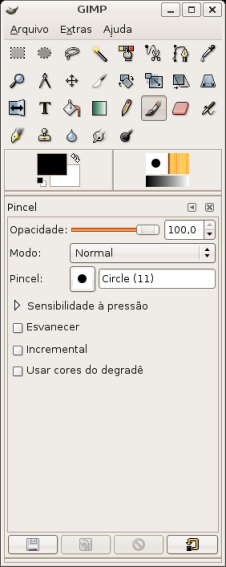
\includegraphics[scale=.7]{gimp-screen}
  \caption{Janela principal do Gimp}
  \label{fig:janela-gimp}
\end{figure}

\begin{figure}[!h]
  \centering
    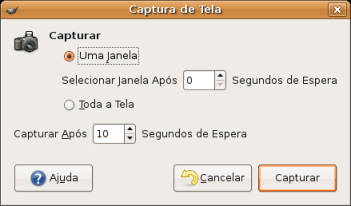
\includegraphics[scale=.7]{captura-gimp-screen}
    \caption{Janela de captura do Gimp}
    \label{fig:captura-gimp}
\end{figure}

Aparecerá a janela da figura \ref{fig:captura-gimp}, na qual pode-se
escolher capturar uma janela ou toda a tela e determinar um tempo de
espera para arrumação.

\subsection{Screenshot via PrintScreen}
\label{sec:scre-via-printscr}

No gerenciador de janelas (window manager) Gnome
\url{http://www.gnome.org/} o uso da tecla printscreen captura toda a
tela.

\part{Programas de áudio}
\label{part:programas-de-audio}

% http://wiki.archlinux.org/index.php/Pro_Audio

You must be in the audio group for user realtime. The file /etc/security/limits.conf should look similar to this:

    * @audio - rtprio 99
    * @audio - nice -10
    * @audio - memlock unlimited 


\chapter{Kernel com suporte para tempo real}
\label{cha:kernel-com-suporte}

%http://irc.esben-stien.name/mediawiki/index.php/Setting_Up_Real_Time_Operation_on_GNU/Linux_Systems

% desabilitar esd no gnome

% >>> You might need to add following line to your /etc/services(without quote):
% >>> "lash       14541/tcp       # LASH client/server protocol"

% >>> Add this line in your /etc/timidity++/timidity.cfg file to enable this soundfont : 
% >>>
% >>> soundfont /usr/share/soundfonts/fluidr3/FluidR3GM.SF2 

% community/jdelay 20060513-3
%     A command line tool to measure JACK audio server latency

% http://lau.linuxaudio.org/faq/index.php/Capabilities
% http://wiki.archlinux.org/index.php/Custom_local_repository
% http://wiki.archlinux.org/index.php/Pro_Audio
% http://bbs.archlinux.org/viewtopic.php?id=30547
% http://www.sound-man.co.uk/linuxaudio/kernel.html
% http://irqbalance.org/
% AlsaMixerGUI
% http://lowlatency.linuxaudio.org/#irq
% http://www.informatik.uni-halle.de/~ladischc/linux_interrupt_priorities.html
% http://www.linuxjournal.com/node/1000262
% http://www.linuxjournal.com/node/1000295
% http://lau.linuxaudio.org/
% http://wiki.drobilla.net/FreePlugins
% http://bristol.sourceforge.net/
% http://64studio.com/quickstart_aeolus
% http://64studio.com/primer_aeolus
% http://64studio.com/quickstart_jack
% http://64studio.com/howto_vst
% http://ladspavst.linuxaudio.org/
% http://rt.wiki.kernel.org/index.php/Main_Page

\chapter{CLM---Common Lisp Music}
\label{cha:clm-common-lisp}

\section{Pré-requisitos}
\label{sec:pre-requisitos}

Para compilar o CLM você precisará do gcc (o compilador C do projeto
GNU) e outras ferramentas instaladas. Além disso, o CLM não é um
programa auto-contido como o Csound. Ele é na verdade uma biblioteca
de funções Lisp. Para utiliza-lo você precisará de um compilador Lisp.
Eu recomendo o SBCL. Finalmente, você precisará de um bom editor. Eu
recomendo o Emacs com o Slime. O comando abaixo deve instalar tudo que
você precisa para começar:

\begin{verbatim}
aptitude install gcc emacs22 slime sbcl csh
\end{verbatim}

\section{Instalação}
\label{sec:instalacao}

Infelizmente não existe um pacote do CLM para o debian, então teremos
que instala-lo manualmente. Além disso, vamos instalar de uma maneira
que é mais fácil mas não é necessariamente robusta. Contudo essa
maneira é suficiente para você iniciar no programa. No futuro veremos
maneiras mais robustas de instalar o CLM.

Baixe a última versão do CLM no site do projeto em
\url{http://ccrma.stanford.edu/software/clm/} e descompacte o tar.gz
em um diretório. O diretório clm-3 será criado quando o arquivo for
descompactado. Os comandos abaixo efetuam essas operações:

\begin{verbatim}
wget ftp://ccrma-ftp.stanford.edu/pub/Lisp/clm-3.tar.gz
tar -xzf clm-3.tar.gz
\end{verbatim}

Em seguida coloque o seguinte código no final do arquivo
\verb|~/.swank.lisp|:

\begin{verbatim}
(defun clm ()
  (require :asdf)
  (setf *clm-dir* #p"/home/kroger/clm-3/")
  (push *clm-dir* asdf:*central-registry*)
  (asdf:operate 'asdf:load-source-op :clm)
  (setf *default-pathname-defaults* *clm-dir*))
\end{verbatim}

Observe que dentro do diretório clm-3 existem diversos arquivos. Os
arquivos com a extensão *.ins definem instrumentos do CLM e são os que
nos interessam. 

Para iniciar o CLM abra o emacs e slime com \texttt{M-x slime}. O REPL
(\textit{Read Eval Print Loop}) é o modo interativo de Lisp. Nele você
pode digitar expressões e obter resultados. Para programas maiores é
desconfortável entrar expressões no REPL, mas para testar coisas ele é
bastante útil. No REPL digite o comando abaixo para iniciar o CLM:

\begin{verbatim}
(clm)
\end{verbatim}

Sempre que você quiser usar o CLM basta iniciar o emacs, carregar o
slime e digitar ``(clm)'' no REPL.

Se você quiser iniciar o slime com uma tecla de atalho, coloque a
linha abaixo no seu \texttt{.emacs}:

\begin{verbatim}
(global-set-key [f9] 'slime)
\end{verbatim}

\section{Uso básico}
\label{sec:uso-basico}

Tendo compilado o CLM você pode carregar e usar instrumentos definidos
nos arquivos *.ins. Por exemplo, o arquivo v.ins define um instrumento
de nome ``fm-violin'' que sintetiza um violino usando FM. Você pode
carregar um instrumento com o comando abaixo:

\begin{verbatim}
(load "v")
\end{verbatim}

Finalmente, você pode usar o instrumento com o comando abaixo:

\begin{verbatim}
(with-sound () (fm-violin 0 1 440 .1)) 
\end{verbatim}

\section{Para saber mais}
\label{sec:para-saber-mais}

Para saber mais sobre a instalação do CLM veja o arquivo README.clm.
O manual está no arquivo clm.html. Ambos estão no diretório do CLM.

\chapter{Nyquist}
\label{cha:nyquist}

\section{Instalação}
\label{sec:instalacao-1}

Para instalar o nyquist é só usar o aptitude:

\begin{verbatim}
aptitude install nyquist
\end{verbatim}

O binário do nyquist se chama \texttt{ny}. Se você digitar \texttt{ny}
no terminal um prompt interativo vai abrir e esperar por comandos.
Você pode digitar algo simples para testar se o programa está
funcionando. O comando abaixo vai tocar um dó central:

\begin{verbatim}
(play (osc 60))
\end{verbatim}

\begin{htmlonly}
  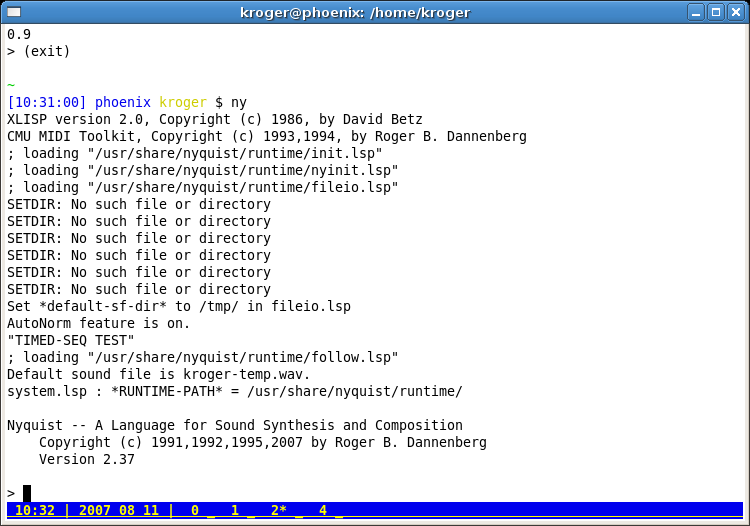
\includegraphics{ny1}
\end{htmlonly}

\begin{latexonly}
  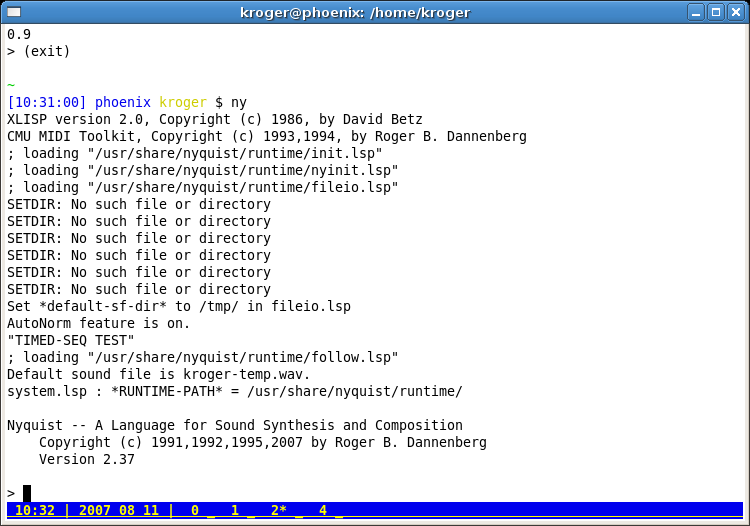
\includegraphics[scale=.5]{ny1}
\end{latexonly}

O manual do nyquist está disponível em
\url{http://www.cs.cmu.edu/~rbd/doc/nyquist/root.html} e em
\url{/usr/share/doc/nyquist/doc/home.html} se você instalou o pacote
debian.

\section{O modo para emacs}
\label{sec:o-modo-para-2}

Um modo preliminar do emacs para o nyquist pode ser encontrado em
\url{http://www.genos.mus.br/handbook/src/inf-nyquist.el}. Baixe o arquivo em
algum lugar no seu computador (eu sugiro \verb|~/lib/emacs/|) e
coloque as seguintes linhas no seu \texttt{.emacs}:

\begin{verbatim}
(autoload 'run-nyquist-lisp   "inf-snd" "Start inferior Snd-Lisp process" t)
(autoload 'nyquist-lisp-mode  "inf-nyquist" "Load nyquist-lisp-mode." t)
(setq inf-nyquist-lisp-program-name "ny")

(add-to-list 'auto-mode-alist '("\\.ny$" . nyquist-lisp-mode))

(add-hook 'nyquist-lisp-mode-hook
          (lambda ()
            (slime-mode nil)
            (local-set-key "\r" 'newline-and-indent)
            (setq lisp-indent-function 'common-lisp-indent-function)
            (setq indent-tabs-mode nil)))
\end{verbatim}

Todos os arquivos com a extensão \texttt{.ny} estarão associados ao
nyquist.

\section{Usando o nyquist com o emacs}
\label{sec:usando-o-nyquist}

Inicie o emacs e abra um arquivo com a extensão \texttt{.ny}, por
exemplo, \texttt{foo.ny}. Observe que o item ``Nyquist'' vai aparecer
no menu. Para iniciar o nyquist escolha no menu Nyquist\sep Start
Nyquist-lisp process ou \texttt{C-c C-s} no teclado. Um buffer chamado
\texttt{*Nyquist-lisp*} será aberto. Esse buffer é o modo interativo
do nyquist.

Você pode digitar comandos do nyquist no arquivo aberto (no nosso caso
\texttt{foo.ny}) e enviá-los para o nyquist com \texttt{C-x C-e} ou
através do menu em Nyquist\sep Send last Sexp.

\begin{htmlonly}
  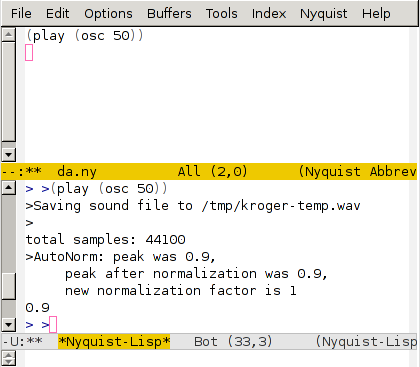
\includegraphics{ny2}
\end{htmlonly}

\begin{latexonly}
  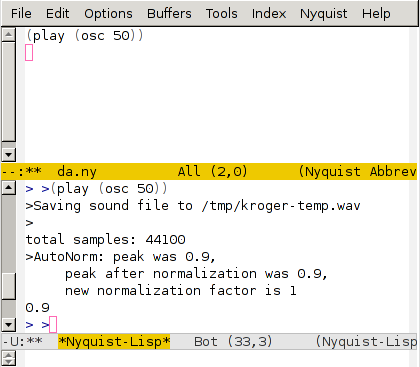
\includegraphics[scale=.5]{ny2}
\end{latexonly}

\section{Desenvolvendo plugins do audacity com o nyquist}
\label{sec:desenv-plug-do}

O audacity tem uma versão do nyquist embutida, de modo que plugins
podem ser desenvolvidos com ele. Os arquivos de plugins devem ser
colocados em \texttt{~/.audacity-files/plug-ins} e o audacity deve ser
reiniciado toda vez que um novo plugin for criado. 

Crie um arquivo \texttt{teste.ny} com o seguinte conteúdo:

\begin{verbatim}
;nyquist plug-in
;version 1
;type process
;name "Teste de fade in"
;action "Fading In..."
(mult (ramp) s)
\end{verbatim}

Observe que o efeito ``Teste de fade in'' vai aparecer no menu de
efeitos do audacity.

Um breve tutorial de como criar plugins do audacity com o nyquist pode
ser visto em \url{http://audacity.sourceforge.net/help/nyquist3}.

\chapter{SuperCollider}
\label{cha:supercollider}

O SuperCollider é uma linguagem de programação para síntese de áudio
em tempo real e composição algorítmica. A página do programa fica em
\url{http://supercollider.sourceforge.net}.

\section{Instalação}
\label{sec:instalacao-2}

Para instalar o supercollider no debian é só executar o comando
abaixo:

\begin{verbatim}
aptitude install supercollider supercollider-doc supercollider-server
\end{verbatim}

\section{Uso básico}
\label{sec:uso-basico-1}

Nós vamos usar o SuperCollider dentro do Emacs. Para ativar o modo
sclang que permite interagir com o SC coloque a seguinte linha no seu
\texttt{~/.emacs}:

\begin{verbatim}
(require 'sclang)
\end{verbatim}

O SuperCollider usar o jack para entrada e saida, então tenha certeza
de te-lo rodando antes de carregar o SC. Inicie o emacs e carregue o
modo sclang:

\begin{verbatim}
M-x sclang-start
\end{verbatim}

O emacs vai abrir dois \textit{buffers}, um chamado *SCLang:Workspace*
e outro *SCLang:PostBuffer*. No Workspace você pode digitar comandos
do SC. Os resultados dos comandos vão aparecer no PostBuffer.

O menu SCLang no emacs tem diversos comandos para lidar com o SC. O
mais importante é como parar um som que esteja tocando. Você pode
acessá-lo em SCLang$\leftarrow$Stop Main no menu, ou pelo teclado com
\texttt{C-c C-s}. Para computar uma linha de código use \texttt{C-c
  C-c } (ou \textit{Evaluate Line} no menu).

Para iniciar o servidor, digite a linha abaixo e, com o cursor em
qualquer lugar da linha, digite \texttt{C-c C-c}:

\begin{verbatim}
s = Server.local.boot;
\end{verbatim}

Agora compute a linha abaixo para tocar um lá continuamente (lembre de
usar o \texttt{C-c C-s} para parar o som).

\begin{verbatim}
{SinOsc.ar(442, 0, 0.2) }.play;
\end{verbatim}

Finalmente, para demonstrar o poder expressivo do SuperCollider, veja
o que é possível de fazer com uma única linha de código:

\begin{verbatim}
play{SinOsc.ar(OnePole.ar(Mix(LFSaw.ar([1,0.99],[0,0.6],2000,2000).trunc([400,600])*[1,-1]),0.98)).dup*0.1};
\end{verbatim}

\section{Para saber mais}
\label{sec:para-saber-mais-1}

O site do SuperCollider tem vários tutoriais na página
\url{http://supercollider.sourceforge.net/learning}.

\chapter{Csound}
\label{cha:csound}

\section{Instalação}
\label{sec:instalacao-4}

Para instalar o csound5 você deve usar o pacote debian do Genos. Veja
a seção \ref{cha:repositorios-debian} para ver como configurar seu
computador para usar o repositório de pacotes do Genos.

Tendo configurado o repositório do genos é só dar o comando abaixo
para instalar o csound.

\begin{verbatim}
aptitude install csound5
\end{verbatim}

Finalmente coloque a linha abaixo no seu \texttt{.bashrc}:

\begin{verbatim}
export OPCODEDIR=/usr/lib/csound/plugins
\end{verbatim}

\section{Uso básico}
\label{sec:uso-basico-2}

Para testar a instalação, crie um arquivo \texttt{teste.orc} com o seguinte
conteúdo:

\begin{verbatim}
instr 1
  a1        oscil     1000,440,1
            out       a1       
endin
\end{verbatim}

Crie também um arquivo \texttt{teste.sco} com o conteúdo abaixo:

\begin{verbatim}
f1  0 1024  10    1

i1 0 3
\end{verbatim}

Para usar o csound no terminal basta digitar \texttt{csound
  <orquestra> <partitura>}, por exemplo:

\begin{verbatim}
csound teste.orc teste.sco
\end{verbatim}

O csound vai gerar um arquivo de áudio chamado \texttt{teste.wav}.
Para ouvir em tempo real use a opção \texttt{-o}:

\begin{verbatim}
csound -odac teste.orc teste.sco
\end{verbatim}

Essa opção também pode ser usada para determinar o nome do arquivo de
áudio da saída:

\begin{verbatim}
csound -o teste.wav teste.orc teste.sco
\end{verbatim}

\section{O modo para emacs}
\label{sec:o-modo-para}

Um modo avançado e completo do csound para emacs está disponível em
\url{www.zogotounga.net/comp/csoundx.html}. Execute o comando abaixo
para baixar e descompactar o arquivo:

\begin{verbatim}
http://www.zogotounga.net/comp/stef-elisp-2.09.zip
unzip stef-elisp-2.09.zip
\end{verbatim}

Em seguida coloque as seguintes linhas no seu \texttt{.emacs}. Não
esqueça de trocar o diretório do comando \texttt{add-to-list} para o
diretório onde você baixou o modo.

\begin{verbatim}
(add-to-list 'load-path "/home/kroger/lib/emacs/stef-elisp/")
(require 'stef-elisp)
\end{verbatim}

A medida que você for customizando seu emacs, pode querer colocar
todas as extensões em um diretório específico. Eu sugiro
\verb|~/lib/emacs|.

\section{Csound com kate}
\label{sec:csound-com-kate}

Kate é um editor para o Kde. Talvez você prefira usa-lo no lugar do
emacs. Primeiro instale-o com o comando abaixo:

\begin{verbatim}
aptitude install kate
\end{verbatim}

Em seguida baixe as definições para csound no link abaixo:

\begin{verbatim}
wget http://flavio.tordini.org/download/kate-csound.zip
\end{verbatim}

Descompacte o arquivo e copie os arquivos .xml para o diretório de
configuração do kate. Se você nunca usou o kate antes, provavelmente
terá que criar o diretório de configuração antes de copiar:

\begin{verbatim}
unzip kate-csound.zip
mkdir -p ~/.kde/share/apps/katepart/syntax
mv csound-*.xml ~/.kde/share/apps/katepart/syntax/
\end{verbatim}

\chapter{Snd}
\label{cha:snd}

\section{Instalação}
\label{sec:instalacao-5}

Para instalar a versão mais nova do snd configure seu computador para
usar o repositório de pacotes debian do genos. Veja como fazer isso na
seção \ref{cha:repositorios-debian}. Para instalar o snd é só digitar
o comando abaixo (como root):

\begin{verbatim}
aptitude install snd
\end{verbatim}

\section{O modo para emacs}
\label{sec:o-modo-para-1}

O snd é um programa para edição de áudio super poderoso. Ele é
completamente customisável usando scheme, um dialeto de lisp. Ele pode
ser controlado a partir do emacs. Para isso, baixe o arquivo
\url{http://www.genos.mus.br/handbook/src/inf-snd.el} para algum lugar no seu
computador (eu sugiro \verb|~/lib/emacs/|) e coloque as seguintes
linhas no seu \texttt{.emacs}:

\begin{verbatim}
(autoload 'run-snd-scheme   "inf-snd" "Start inferior Snd-Scheme process" t)
(autoload 'snd-scheme-mode  "inf-snd" "Load snd-scheme-mode." t)
(setq inf-snd-scheme-program-name "snd")

(add-to-list 'auto-mode-alist '("\\.snd$" . snd-scheme-mode))

(add-hook 'snd-scheme-mode-hook
          (lambda ()
            (local-set-key "\r" 'newline-and-indent)
            (setq lisp-indent-function 'common-lisp-indent-function)
            (setq indent-tabs-mode nil)))
\end{verbatim}

\section{Uso básico com o emacs}
\label{sec:uso-basico-3}

Inicie o jack e o emacs. Depois que o emacs iniciar, execute o comando

\begin{verbatim}
A-x run-snd-scheme
\end{verbatim}

Esse comando vai abrir o scheme e um modo interativo dentro do emacs.
Dentro do emacs abra um arquivo novo com a extensão \texttt{.snd}, por
exemplo, \texttt{teste.snd}. Observe que vai aparecer o menu
\texttt{Snd/Scheme} no menu do emacs. Como o snd tem o CLM embutido,
você pode fazer coisas semelhantes à seção \ref{cha:clm-common-lisp}.
Mas tenha em mente que no CLM estamos usando Common Lisp enquanto no
Snd estamos usando Scheme. Os dois são parecidos (são dialetos de
lisp) mas nem tudo que funciona em um funciona no outro. No arquivo
\texttt{teste.snd} digite o código abaixo:

\begin{verbatim}
(load-from-path "v.scm")
(with-sound () (fm-violin 0 3 440 .1))
\end{verbatim}

Você pode computar cada expressão no menu em Snd/Scheme\sep Send last
Sexp, ou usar \texttt{C-x C-e}. Observe que quando você carregar o
arquivo \texttt{v.ins} ele vai aparecer automaticamente no snd. Você
pode tocar o arquivo com \texttt{C-c C-p} e parar de tocar com
\texttt{C-c C-t}.

Você pode usar a função \texttt{do} para tocar um arpejo:

\begin{verbatim}
(with-sound ()
  (do ((i 0 (1+ i)))
      ((= i 8))
    (fm-violin (* i .25) .5 (* 100 (1+ i)) .1)))
\end{verbatim}

Assim como o CLM, os instrumentos são definidos com
\texttt{definstrument}. O instrumento abaixo toca uma senóide simples:

\begin{verbatim}
(definstrument (simp beg dur freq amp)
  (let* ((os (make-oscil freq))
   (start (seconds->samples beg))
   (end (+ start (seconds->samples dur))))
    (run
      (lambda ()
        (do ((i start (1+ i))) 
            ((= i end))
          (outa i (* amp (oscil os)) *output*))))))
\end{verbatim}

Para tocar o instrumento é só chamar a função \texttt{simp}:

\begin{verbatim}
(with-sound () (simp 0 3 440 .1))
\end{verbatim}

\chapter{Pure Data}
\label{cha:pure-data}

PD (Pure Data) é um ambiente gráfico de programação para áudio, vídeo
e processamento gráfico. Ele é um software livre pode ser baixado para
diversas plataformas, incluindo Linux, Windows, e Mac. O melhor lugar
para começar é o portal do PD em \url{http://puredata.info}

\section{Instalando o PD}

Para instalar o PD no debian é só digitar:

\begin{verbatim}
aptitude install puredata pd-zexy
\end{verbatim}

O debian vem com uma versão básica do PD. O
\htmladdnormallink{pd-extended}
{http://autobuild.puredata.info/auto-build/latest} é uma versão mais
completa, mas ainda está em desenvolvimento.

Para ser produtivo com o PD é recomendado que você instale pacotes
extras, como \textit{externals} e extensões.

Talvez você tenha que colocar a seguinte linha no seu ~/.bashrc

\begin{verbatim}
 export LADSPA_PATH=/usr/lib/ladspa/
\end{verbatim}

Se voce está interessado em compilar tudo a partir do código-fonte, a
página em \url{http://puredata.org/docs/developer/Debian} mostra como
fazer isso no Debian.

\part{Outros programas}
\label{part:outros-programas}

\chapter{Inkscape}
\label{cha:inkscape}

O Inkscape (\url{http://www.inkscape.org}) é um programa para
ilustração vetorial. Utiliza o formato livre .svg, compatível com
softwares livres (Sodipodi) e proprietários (CorelDRAW).

\chapter{Gimp}
\label{cha:gimp}

O Gimp (\url{http://www.gimp.org/}) é um editor de imagens.

\part{Administração}
\label{part:administracao}

\chapter{Máquinas do GenosLab}
\label{cha:maquinas-do-genoslab}

\section{Tutorial de instalação e sincronização de sistema}
\label{sec:tutor-de-inst}

\begin{enumerate}
\item Verificar partições das máquinas
\item Instalar o ArchLinux a partir do cd com pacotes básicos
\item Configurar rc.conf (host e eth0)
\item Configurar hosts.deny
\item Inserir senha de root
\item Atualizar pacotes: \verb!pacman -Sy!
\item Instalar git e rsync
\item Levantar ssh: \verb!/etc/rc.d/sshd start!
\item Colocar /etc em controle de versão (fazer commit a cada passo dado)
\item Baixar pacotes de outra máquina para \verb!/var/cache/pacman/pkg/!
\item Baixar repositório genos-utils em \verb!/root/!:
\item Instalar pacotes genos-base: \verb!pacman -S $(cat /root/genos-utils/manutencao/genos-base.txt)!
\item Copiar preâmbulo e daemons de
  \verb!/root/genos-utils/manutencao/etc/rc.conf.template! para \verb!/etc/rc.conf!
\item Copiar configuração de gdm:
  \verb!cp /root/genos-utils/manutencao/etc/custom.conf /etc/gdm/!
\item Configurar locale:
  \verb!cp /root/genos-utils/manutencao/etc/locale.gen /etc! e rodar
  \verb!locale-gen!
\item Remove configurações do gnome de todos os usuários: \verb!rm -r /home/*/.{gnome*,gconf*}!
\item Verificar permissões de usuários
\item Verificar se \verb!/shared/arch/! está atualizada
\item Ajustar relógio \verb!ntpdate ntp.on.br!
\item Configurar kernelrt no grub
\item Baixar abs: \verb!abs!
\item Alterar limite para ardour. Colocar unlimited em memlock em
  \verb!/etc/security/limits.conf!
\end{enumerate}

\section{Particionamento das máquinas}
\label{sec:part-das-maqu}

As partições das máquinas do Genos estão nas tabelas
\ref{tab:part-tesla}, \ref{tab:part-bohr} e \ref{tab:part-newton}.

\begin{table}[h]
  \centering
  \begin{tabular}{llr}
    Dispositivo & Ponto de montagem & Tamanho \\
    \hline
    sda1 & /boot & 99 MB \\
    sda2 & swap & \\
    sda3 & / & 20 GB \\
    sda4 & /home & 446 GB \\
    sdb1 & /shared & 466 GB \\
  \end{tabular}
  \caption{Partições do Tesla}
  \label{tab:part-tesla}
\end{table}

\begin{table}
  \centering
  \begin{tabular}{llr}
    Dispositivo & Ponto de montagem & Tamanho \\
    \hline
    sda1 & /boot & 274 MB \\
    sda2 & / & 28 GB \\
    sda3 & swap & \\
    sda4 & /home & 436 GB \\
  \end{tabular}
  \caption{Partições do Bohr}
  \label{tab:part-bohr}
\end{table}

\begin{table}
  \centering
  \begin{tabular}{llr}
    Dispositivo & Ponto de montagem & Tamanho \\
    \hline
    sda1 & /boot & 183 MB \\
    sda2 & / & 28 GB \\
    sda3 & /home & 87 GB \\
    sdb1 & /shared & 113 GB \\
    sdb2 & swap & \\
  \end{tabular}
  \caption{Partições do Newton}
  \label{tab:part-newton}
\end{table}

\end{document}
